% Chapter 4
\chapter{روش پیشنهادی برای جابه‌جایی مدل‌های شبکه عصبی بین کاربران}

\section{مقدمه}
در فصل گذشته، به بررسی روش‌های گوناگون برای مقابله با مشکل داده‌های 
\lr{non-IID}
در یادگیری فدرال پرداخته شد. در این فصل، تلاش خواهد شد با استفاده از جابه‌جایی مدل‌های شبکه عصبی بین کاربران نهایی، راهکاری برای پیاده‌سازی یادگیری فدرال بر روی داده‌های 
\lr{non-IID}
ارائه شود. شکل 
\ref{iid_vs_noniid}
به‌خوبی مفهوم داده‌های 
\lr{non-IID}
را توضیح می‌دهد، اما برای این که روشن شود چگونه جابه‌جایی مدل‌ها می‌توانند در این زمینه مؤثر باشند، در این بخش یک مثال مناسب ارائه می‌شود.

فرض کنید که هدف، آموزش مدلی برای شناسایی اشیائی مانند علائم ترافیکی و تابلوهای فروشگاهی است. اگر وسایل نقلیه، یکی در بزرگراه و دیگری در مرکز شهر حرکت کنند، داده‌های ویدیویی آن‌ها توزیع‌های متفاوتی از این علائم و تابلوها را ثبت خواهند کرد. به این صورت که داده‌های جمع‌آوری شده از بزرگراه، احتمالاً تابلوهای فروشگاهی کمتری را شامل می‌شود، در حالی که داده‌های ثبت شده در مرکز شهر حاوی تعداد بیشتری از هر دو نوع علائم و تابلوها هستند. این اختلاف توزیع داده‌ها در دستگاه‌های مختلف، می‌تواند منجر به مشکل انحراف در وزن‌دهی مدل شود.

برای حل این مسئله در پژوهش‌های پیشین، عملیات جابه‌جایی مدل‌های شبکه عصبی بین کاربران پیشنهاد شده است. این رویکرد، مدل‌ها را بین دستگاه‌های نهایی جابه‌جا می‌کند تا تنوع داده‌ها در دستگاه‌های مختلف کاهش یابد. این فرایند با تحمیل هزینه اندک به منابع محاسباتی و ارتباطی، باعث بهبود مدل در برخورد با داده‌های  
\lr{non-IID}  
می‌شود.

در این فصل، ابتدا به معرفی روش جابه‌جایی مدل‌ها پرداخته می‌شود که شامل دو نوع جابه‌جایی تصادفی و بر پایه شباهت است. روش جابه‌جایی بر ‎پایه شباهت، در واقع همان رویکرد پیشنهادی این پژوهش محسوب می‌شود.
سپس، تاثیرات این جابه‌جایی‌ها بر ترافیک شبکه و حفظ حریم شخصی، مورد بررسی قرار می‌گیرد. در ادامه، معیارهای مشابهت و پایداری آن‌ها تعریف و ارزیابی می‌شوند. در پایان، شاخص‌های مشابهت بین شبکه‌های عصبی مشخص شده و دو روش اصلی برای انتخاب کاربران جهت جابه‌جایی مدل‌ها تحلیل می‌شوند.

%در این فصل، ابتدا به مرور روش پیشین جابه‌جایی مدل‌ها پرداخته می‌شود که این روش با عنوان روش جابه‌جایی تصادفی شناخته می‌شود. پس از آن روش پیشنهادی در این پژوهش با عنوان جابه‌جایی بر پایه شباهت معرفی می‌شود. در ادامه، تاثیرات هر یک از این روش‌ها بر ترافیک شبکه و حفظ حریم شخصی، مورد بررسی قرار می‌گیرد. علاوه بر این، معیارهای مشابهت و پایداری آن‌ها تعریف و ارزیابی می‌شوند. در پایان، شاخص‌های مشابهت بین شبکه‌های عصبی مشخص شده و دو روش اصلی برای انتخاب کاربران جهت جابه‌جایی مدل‌ها تحلیل می‌شوند.

\section{
	روش جابه‌جایی فدرال%
	\LTRfootnote{Federated Swapping}
	\lr{\texttt{\fontspec{Times New Roman} (FedSwap)}}
}
در این روش، یک عملیات جدید به نام جابه‌جایی فدرال یا
\lr{FedSwap}
پیشنهاد شده است که به عنوان جایگزینی برای برخی از دوره‌های
\lr{FedAvg}
در یادگیری فدرال به کار می‌رود.
این عملیات با هدف بهبود فرآیند یادگیری فدرال و کاهش تاثیرات منفی داده‌های
\lr{non-IID}
طراحی شده است
\cite{chiu2020semisupervised}.


در روش‌ یادگیری فدرال، پس از هر تکرار، مدل‌های محلی از دستگاه‌های نهایی جمع‌آوری شده و یک مدل جامع از ترکیب آن‌ها ساخته می‌شود. اما در روش
\lr{FedSwap}%
، به‌جای این که این ادغام در هر تکرار انجام شود، سرور مدل‌های محلی را در گام‌های مشخصی بین دستگاه‌ها جابه‌جا می‌کند. در واقع، در انتهای برخی مراحل، عملیات جابه‌جایی و در انتهای برخی دیگر، ادغام مدل‌ها صورت می‌گیرد. این مراحل بر اساس پارامترهایی که به عنوان ورودی تعریف می‌شوند، تعیین می‌گردند.
جهت درک بهتر این ساختار به شکل
\ref{federated_swapping}
توجه نمایید.


\begin{figure}[b!]
	\centering
	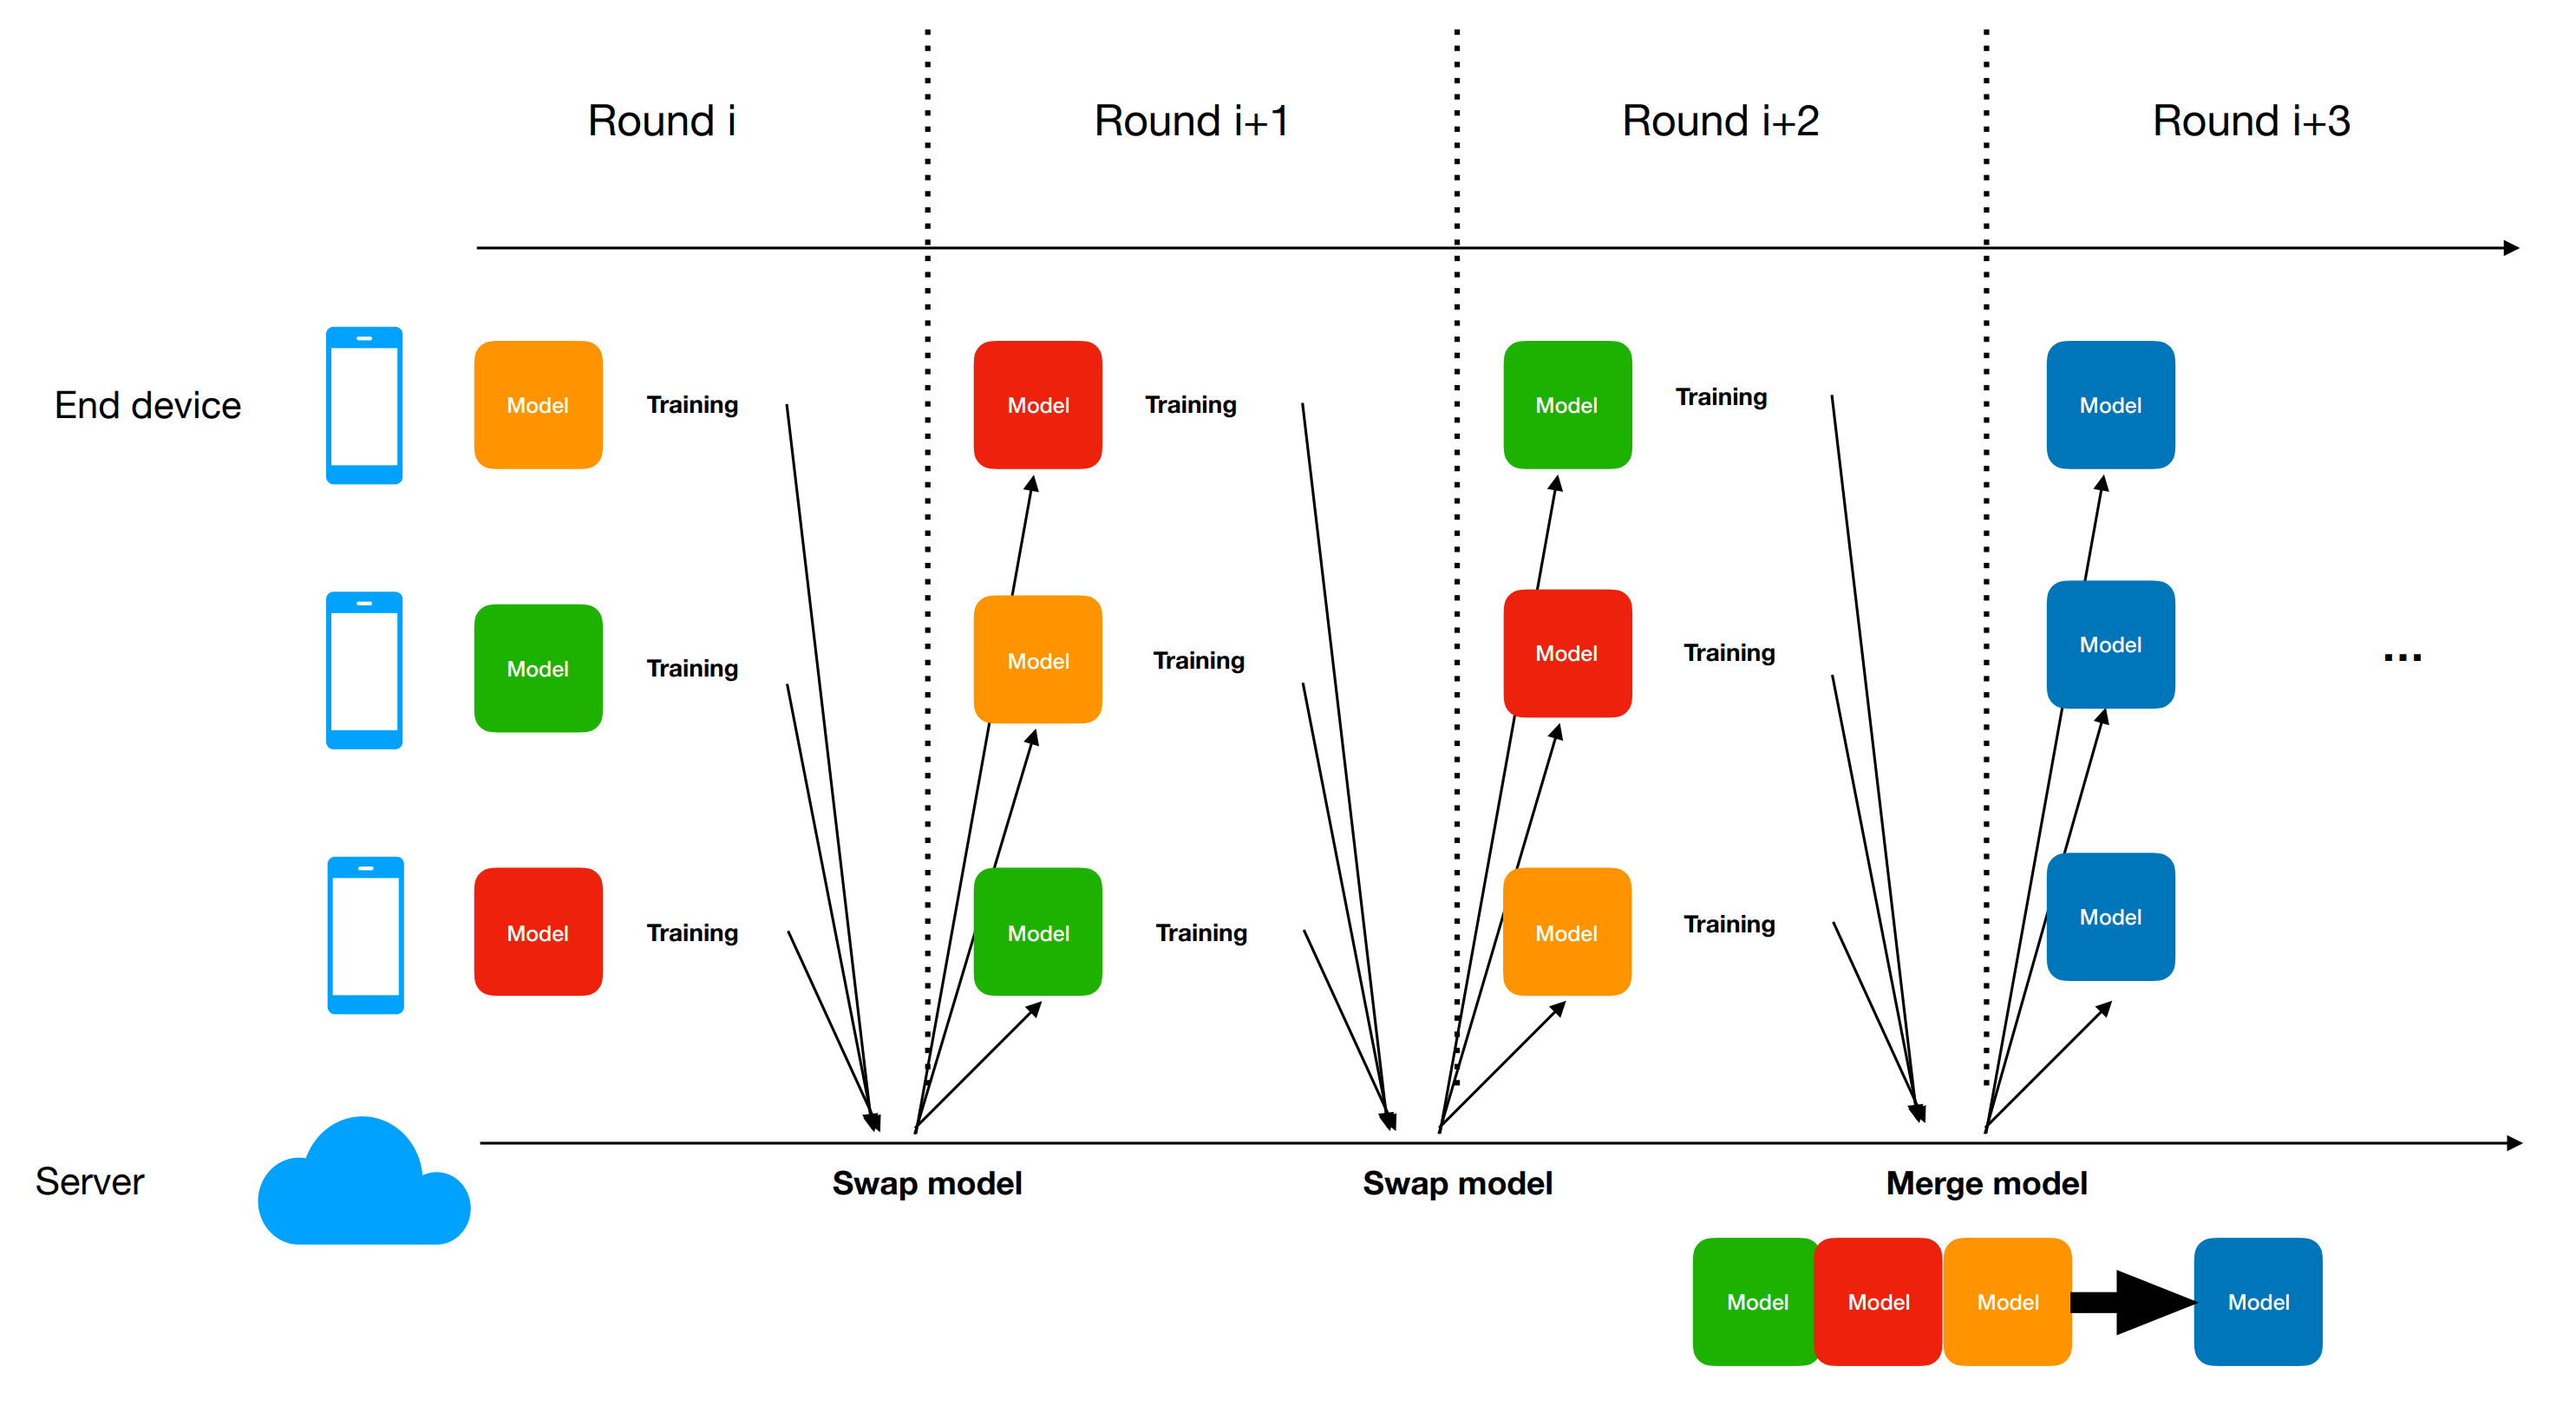
\includegraphics[scale=0.179]{images/chap4/federated_swapping.png}%
	\caption{%
		روش جابه‌جایی فدرال
		\cite{chiu2020semisupervised}%
		.
	}
	\label{federated_swapping}
	\centering
\end{figure}


برای حفظ توازن در این فرآیند، از یک استراتژی چرخشی%
\LTRfootnote{Cyclic}
استفاده می‌شود. در این استراتژی، به‌طور منظم، دو دستگاه نهایی به یکدیگر اجازه می‌دهند که مدل‌های خود را تبادل کنند. این کار باعث می‌شود که همه دستگاه‌های نهایی به‌طور مساوی در فرآیند تبادل مدل‌ها شرکت کنند و هیچ دستگاهی از مزایای این تبادل محروم نماند.

علاوه بر این، انتظار می‌رود که این عملیات جابه‌جایی مدل بین دستگاه‌های نهایی، به هر مدل دید گسترده‌تری از کل مجموعه داده‌ها بدهد. به عبارت دیگر، هر مدل محلی با تبادل مدل با دیگر دستگاه‌ها، می‌تواند اطلاعات بیشتری از داده‌های مختلف دریافت کند. این امر به کاهش انحراف وزن‌ها کمک می‌کند، زیرا مدل‌ها با داده‌های متنوع‌تری آموزش می‌بینند و به تدریج به یک مدل جامع‌تر و دقیق‌تر نزدیک می‌شوند.

به‌طور خلاصه، روش
\lr{FedSwap}
با تبادل مدل‌های محلی بین دستگاه‌های نهایی، نه تنها به بهبود دقت و عملکرد مدل‌ها کمک می‌کند، بلکه مشکلات ناشی از داده‌های
\lr{non-IID}
را نیز کاهش می‌دهد. این روش به عنوان یک رویکرد موثر در یادگیری فدرال می‌تواند باعث بهبود قابل توجهی در نتایج نهایی شود
\cite{chiu2020semisupervised}.


جزئیات عملیات
\lr{FedSwap}
در الگوریتم
\ref{algo_FedSwap}
ارائه شده است.
همچنین در جدول
\ref{tabel_FedSwapNotations}
نمادهای مختص این الگوریتم به نمایش در آمده است.
در این الگوریتم،
$w^k_t$
به عنوان وزن مدل در دستگاه نهایی
$k$
پس از گام
$t$
تنظیم می‌شود. در ابتدا، دستگاه‌های نهایی چندین به‌روزرسانی محلی انجام می‌دهند تا مدل‌های خود را بهبود بخشند. پس از هر
$h_1$
مرحله، سرور وارد عمل شده و عملیات جابه‌جایی را اجرا می‌کند. در این مرحله، مدل‌های محلی بین دستگاه‌های نهایی تبادل می‌شوند تا هر دستگاه بتواند از مدل‌های متنوع‌تری برای آموزش استفاده کند.

این تبادل مدل‌ها به کاهش تنوع داده‌ها بین دستگاه‌های مختلف کمک می‌کند و باعث می‌شود که مدل‌ها با داده‌های مختلفی آموزش ببینند. پس از انجام
$h_2$
عملیات جابه‌جایی، سرور وارد عمل شده و عملیات میانگین‌گیری را اجرا می‌کند. در این مرحله، سرور مدل‌های محلی را تجمیع می‌کند تا یک مدل مشترک ایجاد شود که از داده‌های تمام دستگاه‌ها بهره‌ می‌برد.


\begin{LTR}
	\SetAlgoNlRelativeSize{-1}
	\begin{algorithm}[t]
		\begin{RTL}
			\caption{%
				جابه‌جایی فدرال
				\lr{(FedSwap)}
				\cite{chiu2020semisupervised}
			}
			\label{algo_FedSwap}
		\end{RTL}
		
		\begin{latin}
			Initialize all clients model with weight $w_0$\;
			\For{$t = 1, 2, \ldots, T$}{
				\For{each client $k = 1, 2, \ldots, K$
					\textbf{in parallel}}{
					$w_t^k = w_{t-1}^k - \eta \nabla F(w_{t-1}^k)$\;
				}
				\If{$t|h_1 = 0$ \quad and \quad $t|h_1h_2 \neq 0$}{
					\For{each client $k = 1, 2, \ldots, K$}{
						$w_t^k \gets \texttt{Swapping}(k, \{w_t^k\}_{k \in K})$\;
					}
				}
				\If{$t|h_1h_2 = 0$}{
					$w_t \gets \texttt{WeightedAvg}(\{w_t^k\}_{k \in K})$\;
					\For{each client $k = 1, 2, \ldots, K$
						\textbf{in parallel}}{
						$w_t^k \gets w_t$\;
					}
				}
			}
			\SetKwFunction{Swapping}{Swapping}
			\SetKwFunction{WeightedAvg}{WeightedAvg}
			\SetKwProg{Fn}{Function}{:}{end}
			\Fn{\Swapping{$k, \{w_t^k\}_{k \in K}$}}{
				$r$ \space represent a random client in \space $K$\;
				$w_t \gets w_t^r$\;
				$w_t^r \gets w_t^k$\;
				\KwRet $w_t$\;
			}
			\Fn{\WeightedAvg{$\{w_t^k\}_{k \in K}$}}{
				$w_t \gets \sum_{k=1}^K \frac{n_k}{n} w_t^k$\;
				\KwRet $w_t$\;
			}
		\end{latin}
	\end{algorithm}
\end{LTR}


\begin{table}[h]
	\centering
	\caption{نمادهای مختص الگوریتم
		\lr{FedSwap}
	}
	\label{tabel_FedSwapNotations}
	\begin{tabular}{cr}
		\hline
		متغیر & توضیحات \\
		\hline
		$h_1$ & تعداد گام‌ها بین هر جابه‌جایی \\
		$h_2$ & تعداد جابه‌جایی‌ها بین هر میانگین‌گیری
	\end{tabular}
\end{table}


برای تعیین مقادیر
$h_1$
و
$h_2$%
، ابتدا آزمایش‌های مختلفی انجام شده و بر اساس نتایج به دست آمده به‌صورت تجربی، مقادیر نهایی انتخاب شده‌اند. در این آزمایش‌ها، چند نکته مهم مشاهده شده است. ابتدا، مقدار
$h_1$
به عملکرد به‌روزرسانی مدل محلی در دستگاه‌های نهایی وابسته است. از آن‌ جایی که وظیفه یادگیری معمولاً یک وظیفه عمومی مثل طبقه‌بندی است، مقدار
$h_1$
بر اساس مقدار گام تعریف‌شده در روش میانگین‌گیری فدرال سنتی تنظیم می‌شود
\cite{chiu2020semisupervised}.

علاوه بر این، مقدار
$h_2$
نقش مهمی در توازن بین سربار ارتباطی و همگرایی مدل ایفا می‌کند. با افزایش مقدار
$h_2$%
، تعداد دفعات جابه‌جایی فدرال بین دستگاه‌های نهایی بیشتر خواهد شد. این امر می‌تواند با کاهش تعداد دفعات ادغام فدرال، صرفه‌جویی بیشتری در پهنای باند ارتباطی ایجاد کند. با این حال، این امر ممکن است باعث افزایش احتمال انحراف وزن‌ها و کاهش دقت همگرایی مدل سراسری شود. به عبارت دیگر، هرچه مقدار
$h_2$
بزرگتر باشد، تعداد دفعاتی که مدل‌ها بین دستگاه‌های نهایی جابه‌جا می‌شوند بیشتر است و این ممکن است به بهبود عملکرد مدل‌ها در مواجهه با داده‌های
\lr{non-IID}
کمک کند، اما ریسک انحراف وزن‌ها نیز بیشتر خواهد شد، زیرا مرحله ادغام مدل‌ها به تاخیر خواهد افتاد.

از سوی دیگر، اگر مقدار
$h_2$
کوچکتر باشد، فراوانی جابه‌جایی فدرال بین دستگاه‌های نهایی کاهش می‌یابد. این امر منجر به افزایش سربارهای ارتباطی می‌شود، زیرا نیاز به ادغام مکرر مدل سراسری خواهد بود. بنابراین، مقدار
$h_2$
باید به گونه‌ای تنظیم شود که توازن مناسبی بین کاهش سربار ارتباطی و حفظ دقت مدل ایجاد کند.

در مجموع، روش
\lr{FedSwap}
با جابه‌جایی مدل‌های محلی بین دستگاه‌های نهایی بدون نیاز به هزینه‌های محاسباتی و ارتباطی اضافی، می‌تواند به بهبود عملکرد مدل‌ها در مواجهه با داده‌های
\lr{non-IID}
کمک کند
\cite{chiu2020semisupervised}.



\section{نحوه جابه‌جایی مدل‌ها در یادگیری فدرال}
در این بخش، دو روش متفاوت برای جابه‌جایی مدل‌ها در یادگیری فدرال مورد بررسی قرار می‌گیرد. روش جابه‌جایی تصادفی که مدل‌ها را بر حسب تصادف بین دستگاه‌ها جابه‌جا می‌کند و روش مبتنی بر شباهت که با مقایسه مدل‌ها بر اساس شباهت‌ها و تفاوت‌ شبکه‌های عصبی، تصمیم به مبادله می‌گیرد. هر دو روش به منظور ارتقای عملکرد مدل‌ها در شرایطی که داده‌ها
\lr{non-IID}
هستند، طراحی شده‌اند.

\subsection{
روش جابه‌جایی فدرال به‌صورت تصادفی
}

در الگوریتم
\lr{FedSwap}%
، مدل‌های محلی به‌طور کاملاً تصادفی بین دستگاه‌های نهایی مبادله می‌شوند. به بیان دیگر، هر بار که قرار است دو دستگاه مدل‌های خود را با یکدیگر مبادله کنند، انتخاب این دستگاه‌ها به‌صورت تصادفی صورت می‌گیرد. این باعث می‌شود که هیچ الگوی ثابتی در جابه‌جایی مدل‌ها وجود نداشته باشد و در هر مرتبه، ترکیب جدیدی از دستگاه‌ها در فرآیند تبادل مدل‌ها شرکت کنند.


یکی از ویژگی‌های مهم الگوریتم
\lr{FedSwap}%
، این است که تمام دستگاه‌های نهایی به‌صورت مساوی در فرآیند جابه‌جایی شرکت می‌کنند. به عبارت دیگر، همه دستگاه‌های شرکت کننده در این مرحله از اجرا، در فرآیند جابه‌جایی قرار می‌گیرند، اما انتخاب دستگاه‌ها برای جابه‌جایی به‌صورت تصادفی صورت می‌پذیرد. این باعث می‌شود که تمامی دستگاه‌ها فرصت مساوی برای تبادل مدل‌ها و بهبود دقت و عملکرد خود داشته باشند.

با استفاده از این رویکرد، الگوریتم
\lr{FedSwap}
قادر است به بهبود عملکرد مدل‌های محلی کمک کند، زیرا تبادل تصادفی مدل‌ها بین دستگاه‌ها باعث می‌شود که هر دستگاه به داده‌ها و اطلاعات بیشتری دسترسی پیدا کند. این امر به کاهش انحراف وزن‌ها و بهبود همگرایی مدل سراسری کمک می‌کند.


\subsection{
روش پیشنهادی جابه‌جایی فدرال بر پایه شباهت%
	\LTRfootnote{Similarity-based Federated Swapping}
	\lr{\texttt{\fontspec{Times New Roman} (SimFedSwap)}}%
}
همان‌گونه که پیش‌تر بیان شد، هدف اصلی این پژوهش، انتخاب دستگاه‌های نهایی بر اساس میزان شباهت مدل‌های شبکه عصبی و جابه‌جایی آن‌ها با یکدیگر است. برای این منظور، باید به‌طور کامل با ساختار شبکه عصبی آشنا بوده و مدل‌های مختلف را با یکدیگر مقایسه کرد. این مقایسه امکان ارزیابی میزان شباهت و تفاوت بین مدل‌های شبکه عصبی را فراهم می‌کند.

بعد از بررسی و تعیین میزان شباهت مدل‌ها، باید تصمیم گرفت که کدام یک از آن‌ها را با یکدیگر جابه‌جا نمود. در روش پیشنهادی
\lr{SimFedSwap}
بهترین انتخاب برای جابه‌جایی، مدلی است که کمترین شباهت را با مدل شبکه عصبی دستگاه فعلی دارد. دلیل این انتخاب این است که اگر مدل دستگاه فعلی با مدل دستگاه مقصد شباهت زیادی داشته باشد، جابه‌جایی آن‌ها مؤثر نخواهد بود. این شباهت بالا به این معناست که این دو دستگاه نهایی داده‌های مشابهی داشته و در طول زمان آموزش‌های مشابهی دیده‌اند، در نتیجه جابه‌جایی مدل‌ها تأثیر قابل‌توجهی بر بهبود یادگیری نخواهد داشت.

بنابراین، برای توضیح دلیل ارائه این روش، می‌توان به این نکته اشاره کرد که جابه‌جایی مدل‌هایی که کمترین شباهت را بین دستگاه‌های مختلف دارند، به بهبود فرآیند یادگیری کمک خواهند کرد. این فرض بر این اساس است که دستگاه‌هایی با مدل‌های متفاوت، احتمالاً داده‌هایی با ساختارهای متفاوت دارند. پس جابه‌جایی مدل‌ها بین این دستگاه‌ها، مدل‌ها را با داده‌های جدیدی روبه‌رو می‌کند که می‌تواند به یادگیری بهتر و متنوع‌تر کمک کند. در نتیجه، مدل سراسری سریع‌تر به سمت مسیر بهینه همگرا می‌شود و دقت و کارایی آن افزایش می‌یابد.

این روش نه تنها تنوع داده‌ها را در فرآیند یادگیری افزایش می‌دهد، بلکه به کاهش انحراف وزن‌ها نیز کمک می‌کند. با داشتن دید گسترده‌تری از داده‌ها و تجربیات مختلف، مدل‌ها می‌توانند بهتر و جامع‌تر آموزش ببینند. این امر در نهایت منجر به بهبود عملکرد کلی مدل در شرایط واقعی می‌شود و کمک می‌کند که مدل‌های یادگیری فدرال بتوانند با چالش‌های داده‌های
\lr{non-IID}
به نحو بهتری مقابله کنند.


نحوه مدیریت بار محاسباتی در روش
\lr{SimFedSwap}
به این صورت است که ابتدا تمام مدل‌های شبکه عصبی از دستگاه‌های نهایی به سمت سرور ارسال می‌شوند. سپس سرور بر اساس معیارهای مشخصی، شباهت بین این مدل‌ها را بررسی و اقدام به جابه‌جایی آن‌ها می‌کند. در این روش، تمامی عملیات پردازشی بر روی سرور انجام شده و تصمیم‌گیری درباره تبادل مدل‌ها نیز به عهده سرور خواهد بود. این با فرض محدودیت دستگاه‌های نهایی از لحاظ سخت‌افزار و منابع در دسترس سازگار است.

با انجام عملیات بر روی سرور، دستگاه‌های نهایی تنها به تبادل داده‌های لازم و اجرای به‌روزرسانی‌های محلی سبک می‌پردازند. این رویکرد باعث خواهد شد که فرآیند یادگیری بهینه‌تری ایجاد شود و مدل‌ها به‌طور موثر و کارآمدتری آموزش ببینند. در نتیجه، مشکلات محاسباتی به حداقل می‌رسد و عملکرد کلی سیستم بهبود خواهد یافت.

این روش نه تنها به حفظ منابع محدود دستگاه‌های نهایی کمک می‌کند، بلکه بهره‌وری بالاتری نیز از قدرت پردازشی سرور به دست می‌آید. به این ترتیب، می‌توان اطمینان داشت که عملیات‌های پیچیده و محاسبات سنگین به درستی و با سرعت مناسب انجام می‌شوند، بدون این که فشار اضافی بر دستگاه‌های نهایی وارد شود. به این ترتیب، این روش می‌تواند به‌طور موثری در محیط‌های مختلف با دستگاه‌های متنوع و منابع محدود پیاده‌سازی شود و نتایج قابل اعتمادی ارائه دهد.



\section{
	تعریف معیار مشابهت
}
فرض کنید \( X \) ماتریسی با ابعاد \( n \times p_1 \) باشد که \( X \in \mathbb{R}^{n \times p_1} \) شامل \( n \) نمونه و \( p_1 \) ویژگی است. همچنین، \( Y \) ماتریسی با ابعاد \( n \times p_2 \) باشد که \( Y \in \mathbb{R}^{n \times p_2} \) شامل \( n \) نمونه و \( p_2 \) ویژگی است. فرض می‌شود که \( p_1 \) کمتر یا مساوی \( p_2 \) است.


هدف طراحی و تحلیل یک شاخص شباهت عددی \( s(X, Y) \) است که بتواند بازنمایی‌های%
\LTRfootnote{Representations}
موجود در ماتریس‌های \( X \) و \( Y \) را هم درون یک شبکه عصبی و هم بین شبکه‌های عصبی مختلف مقایسه کند. چنین شاخصی به درک بهتر تأثیر عوامل مختلف در یادگیری عمیق کمک می‌کند.

به عنوان مثال، در بررسی شبکه‌های عصبی، ماتریس \( X \) می‌تواند نمایانگر فعال‌سازهای%
\LTRfootnote{Activations}
نورون‌ها در یک لایه خاص برای \( n \) نمونه ورودی باشد و ماتریس \( Y \) می‌تواند نمایانگر فعال‌سازهای نورون‌ها در لایه‌ای دیگر یا حتی در یک شبکه عصبی دیگر برای همان \( n \) نمونه باشد. مقایسه این دو ماتریس اطلاعات مهمی درباره نحوه یادگیری و بازنمایی داده‌ها توسط شبکه عصبی ارائه می‌دهد.

شاخص \( s(X, Y) \) باید توانایی اندازه‌گیری شباهت‌ها و تفاوت‌های بین بازنمایی‌های مختلف را داشته باشد. این شاخص می‌تواند به پژوهشگران کمک کند تا نحوه تغییر بازنمایی‌ها در اثر عوامل مختلف مانند تغییرات در داده‌های ورودی، تغییرات در معماری شبکه یا تغییرات در پارامترهای آموزش را بهتر درک کنند.

طراحی و تحلیل این شاخص شباهت می‌تواند به درک بهتر از نحوه عملکرد شبکه‌های عصبی کمک نموده و ابزار مفیدی برای بهبود روش‌های آموزش و بهینه‌سازی شبکه‌های عصبی فراهم کند.


\section{
	پایداری در معیارهای مشابهت
}
در این بخش، ویژگی‌های ضروری برای معیارهای مقایسه بازنمایی‌های شبکه عصبی مورد بررسی قرار می‌گیرند. این بررسی شامل تحلیل پایداری شاخص‌های شباهت و تأثیرات آن‌ها در ارزیابی شباهت بازنمایی‌های شبکه عصبی است. همچنین، به اهمیت معیارهای شباهتی پرداخته می‌شود که نسبت به تبدیل‌های متعامد%
\LTRfootnote{Orthogonal Transformation}
و مقیاس‌بندی یکسان%
\LTRfootnote{Isotropic Scaling}
پایدار هستند.
این ویژگی‌ها به معیار شباهت امکان می‌دهند تا بازنمایی‌های شبکه عصبی را به درستی مقایسه کرده و تأثیرات مختلف در فرآیند آموزش شبکه عصبی را بهتر درک کند.


\subsection{پایداری نسبت به تبدیل متعامد}

پایداری نسبت به تبدیل‌های متعامد به این معناست که اگر \( s(X, Y) \) یک شاخص شباهت بین دو ماتریس \( X \) و \( Y \) باشد، این شاخص باید در مقابل تغییرات متعامد نیز پایدار باقی بماند. به عبارت دیگر، اگر \( U \) و \( V \) ماتریس‌های متعامد با رتبه کامل%
\LTRfootnote{Full Rank}
باشند که شرط \( U^TU = I \) و \( V^TV = I \) را برآورده کنند، باید \( s(X, Y) = s(XU, YV) \) باشد. این ویژگی تضمین می‌کند که حتی در صورتی که ابعاد \( p \) بزرگتر از \( n \) باشند، شاخص شباهت همچنان به‌طور مطلوب عمل می‌کند. علاوه بر این، تبدیل‌های متعامد خواص مهمی از جمله حفظ حاصل‌ضرب‌های عددی و فاصله‌های اقلیدسی%
\LTRfootnote{Euclidean Distances}
بین نمونه‌ها را نیز حفظ می‌کنند. این امر باعث می‌شود که مقایسه‌های انجام شده توسط این شاخص‌ها دقیق و قابل اعتماد باشند
\cite{kornblith2019similarity}.

پایداری نسبت به تبدیل‌های متعامد برای شبکه‌های عصبی که با استفاده از روش نزول گرادیان آموزش داده می‌شوند، بسیار مطلوب است. این ویژگی نه تنها پایداری نسبت به تغییرات متعامد را تضمین می‌کند بلکه شامل پایداری نسبت به جایگشت نیز می‌شود. جایگشت در یک ماتریس به معنای این است که مقدارهای درون ماتریس فقط جابه‌جا می‌شوند و ارزش‌های آن‌ها ثابت باقی می‌مانند. این پایداری برای تطبیق تقارن‌های شبکه‌های عصبی ضروری است
\cite{chen1993geometry, orhan2017skip}.

در حالت خطی، اگر ورودی‌ها با یک تبدیل متعامد تغییر کنند، روند آموزش با روش نزول گرادیان تحت تأثیر قرار نمی‌گیرد. برای شبکه‌های عصبی که با وزن‌های متقارن و تصادفی شروع می‌شوند، تبدیل‌های متعامد بر فعال‌سازها باعث می‌شود که روند آموزشی مشابه حالت بدون تغییر باقی بماند. اما اگر یک تغییر خطی دلخواه انجام شود، این ویژگی حفظ نمی‌شود و ممکن است روند آموزش تحت تأثیر منفی قرار گیرد
\cite{lecun1990second}.

به‌طور کلی، پایداری نسبت به تبدیل‌های متعامد در شبکه‌های عصبی اهمیت زیادی دارد زیرا این ویژگی کمک می‌کند تا شبکه‌های عصبی در مواجهه با تغییرات متقارن در داده‌ها، به درستی عمل کنند و دقت و کارایی آن‌ها در فرآیند آموزش بهینه باقی بماند.



\subsection{پایداری نسبت به مقیاس‌بندی یکسان}

شاخص‌های شباهت باید هنگام مقیاس‌بندی یکسان ورودی‌ها، ثابت بمانند. به این معنا که اگر ورودی‌ها در اعداد مثبتی مانند \(\alpha\) و \(\beta\) ضرب شوند، نباید تغییری در شاخص شباهت ایجاد شود. به عبارت دیگر، مقدار \( s(X, Y) \) باید همانند \( s(\alpha X, \beta Y) \) باقی بماند و برای هر \(\alpha\) و \(\beta\) مثبت، درست باشد.

این ویژگی اهمیت خاصی دارد، زیرا تضمین می‌کند که مقایسه بازنمایی‌های شبکه‌های عصبی تحت تأثیر مقیاس‌بندی یکسان قرار نمی‌گیرد و دقت شاخص حفظ می‌شود. در واقع، این شاخص‌ها قادرند در شرایطی که شبکه‌های عصبی تحت تغییرات یکسان مقیاس قرار می‌گیرند، همچنان به درستی بازنمایی‌های مختلف را مقایسه کنند
\cite{kornblith2019similarity}.

به عنوان مثال، وقتی شبکه‌های عصبی در معرض تغییرات یکسان مقیاس قرار می‌گیرند، این شاخص‌ها همچنان قادر خواهند بود بازنمایی‌های مختلف را به درستی مقایسه کنند. این ویژگی امکان فهم بهتر تأثیرات گوناگون در طول آموزش شبکه‌های عصبی و استفاده از این شاخص‌ها برای تحلیل و بهبود عملکرد مدل‌ها را فراهم می‌کند. بنابراین، شاخص‌های مقاوم در برابر مقیاس‌بندی یکسان می‌توانند ابزار مفیدی برای ارزیابی و بهینه‌سازی شبکه‌های عصبی باشند.



\section{مقایسه ساختارهای مشابهت}
یکی از چالش‌های اصلی در تحلیل بازنمایی‌های شبکه‌های عصبی، مقایسه ویژگی‌های چندگانه هر نمونه در بازنمایی‌های مختلف است. این روش ممکن است پیچیده و زمان‌بر باشد و نتایج گمراه‌کننده‌ای ایجاد کند. برای حل این مشکل، می‌توان از رویکردی استفاده کرد که به‌جای مقایسه مستقیم ویژگی‌های هر نمونه، ساختارهای شباهتی بین نمونه‌ها را بررسی کند.

ایده اصلی این است که به‌جای مقایسه مستقیم ویژگی‌های چندگانه هر نمونه در دو بازنمایی مختلف، می‌توان ابتدا شباهت بین هر جفت نمونه در هر بازنمایی را به‌صورت جداگانه سنجید و سپس این ساختارهای شباهتی را با هم مقایسه کرد
\cite{kornblith2019similarity}.

برای درک بهتر این موضوع، تصور کنید که به‌جای مقایسه مستقیم ویژگی‌های چندبعدی دو نمونه، ابتدا میزان شباهت هر یک از این نمونه‌ها به سایر نمونه‌ها بررسی می‌شود. سپس، این ماتریس‌های شباهت، که میزان شباهت هر نمونه به دیگر نمونه‌ها را نشان می‌دهند، با یکدیگر مقایسه می‌شوند.

نکته مهم این است که اگر برای اندازه‌گیری شباهت از ضرب داخلی استفاده شود، شباهت بین ماتریس‌های بازنمایی به یک مفهوم دیگر و قابل درک از شباهت بین ویژگی‌های جفتی تبدیل می‌شود. به عبارت دیگر، این روش امکان دست‌یابی به درک دقیق‌تری از شباهت بین ویژگی‌ها را بدون مقایسه مستقیم ویژگی‌های چندگانه هر نمونه فراهم می‌کند. این رویکرد می‌تواند به‌طور قابل توجهی در تحلیل و درک بازنمایی‌های شبکه‌های عصبی و داده‌های پیچیده مؤثر باشد، زیرا ساختارهای پیچیده را به شیوه‌ای ساده‌تر و قابل فهم‌تر بررسی می‌کند
\cite{kornblith2019similarity}.



\subsection{
	ضرب داخلی%
	\LTRfootnote{Inner Product}
}
یک رابطه ساده وجود دارد که ضرب داخلی بین نمونه‌ها را با ضرب داخلی بین ویژگی‌ها مرتبط می‌سازد:
\begin{equation}
	\langle \text{vec}(XX^T), \text{vec}(YY^T) \rangle = \text{tr}(XX^TYY^T) = ||Y^TX||_F^2
	\label{eq_DotProduct}
\end{equation}
که در آن عناصر \(XX^T\) و \(YY^T\) نشان‌دهنده ضرب داخلی بین بازنمایی نمونه‌های \(i\) و \(j\) هستند و شباهت بین این نمونه‌ها را بر اساس شبکه‌های مربوطه نشان می‌دهند. 

به بیان دیگر، بخش چپ رابطه
\eqref{eq_DotProduct}%
، میزان مشابهت بین الگوهای شباهت، میان نمونه‌ها را ارزیابی می‌کند. این در حالی است که سمت راست، با جمع کردن مربعات ضرب‌های داخلی بین هر جفت از نمونه‌ها، به همان نتیجه مشابه می‌رسد و شباهت بین ویژگی‌های \(X\) و \(Y\) را اندازه‌گیری می‌کند.

این رابطه نشان می‌دهد که می‌توان به‌جای مقایسه مستقیم ویژگی‌ها، از شباهت‌های بین نمونه‌ها استفاده کرد تا به فهم بهتری از بازنمایی‌های شبکه‌های عصبی و داده‌های پیچیده دست یافت. به این ترتیب، تحلیل و درک داده‌ها ساده‌تر و مؤثرتر می‌شود، زیرا این روش امکان دستیابی به نتایج دقیق‌تر را با استفاده از شباهت‌های موجود بین نمونه‌ها به‌صورت غیرمستقیم فراهم می‌کند.




\subsection{
	انتخاب هسته%
	\LTRfootnote{Kernel}
}\label{sec_kernel_selection}
در معیارهای مشابهت و اندازه‌گیری وابستگی، مفهوم هسته یا
\lr{kernel}
نقش بسیار مهمی دارد. هسته در واقع یک تابع ریاضی است که برای محاسبه شباهت بین داده‌های ورودی استفاده می‌شود. این تابع، داده‌ها را به یک فضای ویژگی بالاتر نگاشت می‌کند تا بتوان همبستگی‌ها و مشابهت‌های پیچیده‌تر بین آن‌ها را بهتر سنجید.



به بیان ساده‌تر، تابع هسته \( k \) یک تابع مثبت معین است که دو بردار ورودی \( x_i \) و \( x_j \) را گرفته و یک عدد حقیقی تولید می‌کند که نشان‌دهنده میزان شباهت بین این دو بردار است. هسته‌ها می‌توانند به شکل‌های مختلفی باشند که هر کدام ویژگی‌ها و کاربردهای خاص خود را دارند. در این‌جا با اقتباس از
\cite{kornblith2019similarity}
به چند نمونه رایج اشاره می‌شود.

\begin{itemize}
\item
هسته خطی%
\LTRfootnote{Linear Kernel}:
این هسته به سادگی ضرب داخلی دو بردار ورودی را محاسبه می‌کند.
\begin{equation}
	k(x_i, x_j) = x_i^T x_j
\end{equation}
	
	
	
\item 
هسته چندجمله‌ای%
\LTRfootnote{Polynomial Kernel}:
این هسته ضرب داخلی را با یک توان مثبت، بالا می‌برد.
\begin{equation}
	k(x_i, x_j) = (x_i^T x_j + c)^d
\end{equation}
که در آن \( c \) یک ثابت و \( d \) درجه چندجمله‌ای است.

	
\item
هسته گاوسی
\lr{(RBF)}%
\LTRfootnote{Radial Basis Function Kernel}:
این هسته فاصله اقلیدسی بین دو بردار را در یک تابع نمایی قرار می‌دهد که باعث می‌شود داده‌هایی که نزدیک به هم هستند شباهت بیشتری داشته باشند.
\begin{equation}
	k(x_i, x_j) = \exp\left(-\frac{||x_i - x_j||^2}{2\sigma^2}\right)
\end{equation}
که در آن \( \sigma \) پارامتر پهنای باند و تنظیم‌کننده میزان تاثیر فاصله می‌باشد.
\end{itemize}

برای هسته
\lr{RBF}%
، چندین استراتژی مختلف برای انتخاب پهنای باند \(\sigma\) وجود دارد که میزان تأکید بر شباهت فواصل کوچک نسبت به فواصل بزرگ را کنترل می‌کند. پارامتر \(\sigma\) به عنوان کسری از فاصله میانه، بین نمونه‌ها تنظیم می‌شود. در عمل، مشاهده می‌شود که هسته‌های
\lr{RBF}
و خطی در بیشتر آزمایش‌ها نتایج مشابهی ارائه می‌دهند
\cite{kornblith2019similarity}.

استفاده از توابع هسته‌ای در معیارهای مشابهت و وابستگی، این امکان را فراهم می‌کند که داده‌های ورودی به یک فضای ویژگی بالاتر نگاشت شوند، جایی که روابط پیچیده و غیرخطی بین داده‌ها می‌توانند به‌صورت ساده‌تری مدل‌سازی شوند. به این ترتیب، معیارها با بهره‌گیری از هسته‌ها می‌توانند تحلیل دقیق‌تر و کارآمدتری از داده‌های پیچیده ارائه دهند. این ویژگی باعث می‌شود که هسته‌ها ابزار قدرتمندی در تحلیل داده‌ها باشند.



\section{
	معیار‌های سنجش مشابهت
}\label{sec_similarity_measurement_criteria}
در این بخش به بررسی روش‌های مختلفی که برای سنجش مشابهت بین بازنمایی‌های شبکه‌های عصبی استفاده می‌شود، پرداخته خواهد شد. یکی از روش‌های مهم در این زمینه استفاده از پایه‌های متعامد است. به‌طور خاص، فرض می‌شود که \( Q_X \) و \( Q_Y \) پایه‌های متعامدی برای ستون‌های ماتریس‌های \( X \) و \( Y \) هستند. به این معنا که \( Q_X \) و \( Q_Y \) به‌صورت \( Q_X = X(X^T X)^{-1/2} \) و \( Q_Y = Y(Y^T Y)^{-1/2} \) تعریف شده‌اند. این پایه‌های متعامد امکان تحلیل مؤثرتر بازنمایی‌های شبکه عصبی و سنجش دقیق‌تر شباهت‌های آن‌ها را فراهم می‌کنند.
تمامی رابطه‌های مورد استفاده در بخش
\ref{sec_similarity_measurement_criteria}%
، از مرجع 
\cite{kornblith2019similarity} 
برگرفته شده‌اند.


استفاده از پایه‌های متعامد این امکان را فراهم می‌کند که بدون نگرانی از وابستگی‌های خطی بین ستون‌ها، شباهت‌ها به‌صورت مستقیم مقایسه شوند. این رویکرد به ویژه زمانی مفید است که هدف بررسی نحوه استخراج و بازنمایی ویژگی‌های مختلف داده‌ها توسط شبکه عصبی باشد. با این روش، می‌توان تحلیل‌های دقیقی انجام داد تا تأثیر تغییرات در داده‌های ورودی یا ساختار شبکه بر بازنمایی‌های داخلی بهتر درک شود. چنین تحلیل‌هایی می‌توانند در بهبود و بهینه‌سازی شبکه‌های عصبی و الگوریتم‌های یادگیری عمیق نقش بسزایی داشته باشند.


\subsection{
	قرینه مجموع اختلاف مطلق%
	\LTRfootnote{Opposite Sum of Absolute Difference}
	\lr{\texttt{\fontspec{Times New Roman} (OSAD)}}
}
معیار سنجش شباهت باید به گونه‌ای تعریف شود که علاوه بر داشتن پایداری در مقابل تبدیل‌های متعامد و مقیاس‌بندی یکسان، قادر باشد ماتریس‌هایی با ابعاد مختلف را نیز پوشش دهد. با این حال، در صورتی که فرض شود ماتریس‌های مورد بررسی دارای ساختار یکسان و ابعاد ثابت هستند و همچنین مقدار‌های اولیه این ماتریس‌ها یکسان در نظر گرفته شوند، می‌توان از معیار
\lr{OSAD}
استفاده نمود.

در صورتی که ابعاد به شکل \( n \times p \) تعریف شوند، از رابطه زیر برای مقایسه و اندازه‌گیری شباهت استفاده می‌شود:
\begin{equation}
	OSAD = -\sum_{i=1}^n \sum_{j=1}^{p_1} Z_{ij}
	\quad \text { where } \quad
	Z = |X-Y|
\end{equation}

در این رابطه، \( X \) و \( Y \) ماتریس‌های ورودی هستند و \( Z \) ماتریسی است که از اختلاف مطلق بین این دو به دست می‌آید. در نهایت قرینه مجموع مقادیر ماتریس \( Z \) که با
\lr{OSAD}
نشان داده می‌شود، به عنوان معیاری برای سنجش میزان شباهت مورد استفاده قرار می‌گیرد.

با توجه به این که در این روش فرض بر این است که ابعاد ماتریس‌ها و مقدار‌های اولیه ثابت و یکسان هستند، معیار
\lr{OSAD}
به عنوان ابزاری مفید و قابل اعتماد برای مقایسه و ارزیابی شباهت بین دو ماتریس مختلف مطرح می‌شود. این معیار به سادگی اختلاف‌های موجود در مقادیر را محاسبه کرده و قرینه مجموع آن‌ها را به عنوان نتیجه ارائه می‌دهد، که در تحلیل‌های مختلف بسیار کاربردی خواهد بود.




\subsection{
	تحلیل همبستگی کانونی%
	\LTRfootnote{Canonical Correlation Analysis}
	\lr{\texttt{\fontspec{Times New Roman} (CCA)}}
}
برای درک بهتر تحلیل همبستگی کانونی، از یک مثال ساده استفاده می‌شود. فرض کنید دو مجموعه داده مختلف در اختیار است، مجموعه‌ای شامل اطلاعاتی همچون قد و وزن افراد و مجموعه دیگر حاوی اطلاعاتی مانند سن و درآمد آن‌ها باشد. هدف تحلیل همبستگی کانونی، این است که ارتباط‌های پنهان بین این دو مجموعه داده را کشف کند. به بیان ساده،
\lr{CCA}
به دنبال شناسایی ترکیب‌هایی از ویژگی‌ها در هر مجموعه داده است که با مقایسه آن‌ها، بیشترین همبستگی حاصل شود. تلاش بر این است که مشخص شود کدام ترکیب قد و وزن با کدام ترکیب سن و درآمد بیشترین ارتباط را دارد.

ابتدا داده‌ها استاندارد می‌شوند، به این صورت که میانگین هر ویژگی صفر شده و داده‌ها به گونه‌ای تغییر می‌کنند که انحراف معیارشان یک شود. سپس،
\lr{CCA}
بردارهای وزنی را برای هر مجموعه داده محاسبه می‌کند تا ترکیب‌های خطی از این داده‌ها ایجاد کند. این ترکیب‌ها به گونه‌ای انتخاب می‌شوند که حداکثر همبستگی بین آن‌ها وجود داشته باشد. به عنوان مثال،
\lr{CCA}
می‌خواهد ترکیبی از قد و وزن (مثلاً \(0.5 \times \text{قد} + 0.5 \times \text{وزن}\)) و ترکیبی از سن و درآمد (مثلاً \(0.3 \times \text{سن} + 0.7 \times \text{درآمد}\)) را بیابد که بیشترین ارتباط را با هم داشته باشند.

با استفاده از این بردارهای وزنی، ترکیب‌های جدیدی از داده‌ها ایجاد می‌شوند و سپس همبستگی بین این ترکیب‌ها محاسبه می‌شود.
\lr{CCA}
به دنبال یافتن پایه‌هایی برای دو ماتریس است به طوری که وقتی ماتریس‌های اصلی بر روی این پایه‌ها توزیع می‌شوند، همبستگی به حداکثر برسد. برای هر \(i\) که بین 1 تا \(p_1\) (تعداد ویژگی‌ها) قرار دارد، ضریب همبستگی کانونی \( \rho_i \) به‌صورت زیر تعریف می‌شود: 
\begin{equation}
	\rho_i = \max_{\mathbf{w}_X^i, \mathbf{w}_Y^i} \text{corr}(X \mathbf{w}_X^i, Y \mathbf{w}_Y^i)
\end{equation}
با در نظر گرفتن بردارهای \(\mathbf{w}_X^i \in \mathbb{R}^{p1}\) و \(\mathbf{w}_Y^i \in \mathbb{R}^{p2}\)، ضریب همبستگی کانونی \( \rho_i \) هدفش این است که همبستگی بین ترکیب خطی \( X \mathbf{w}_X^i \) و \( Y \mathbf{w}_Y^i \) را به حداکثر برساند.

برای اطمینان از این که ترکیب‌های جدید داده‌ها مستقل و متفاوت از هم باشند، شرط‌های زیر باید رعایت شوند:
\begin{equation}
	\begin{array}{ll}
		\forall_{j<i} & X \mathbf{w}_X^i \perp X \mathbf{w}_X^j
		\\
		\\
		\forall_{j<i} & Y \mathbf{w}_Y^i \perp Y \mathbf{w}_Y^j
	\end{array}
\end{equation}
این شرط‌ها اطمینان می‌دهند که ترکیب‌های جدید از داده‌ها با ترکیب‌های قبلی همپوشانی نداشته و متعامد باقی بمانند.

در نهایت برای مقایسه دو شبکه عصبی و اندازه‌گیری شباهت بین آن‌ها، از معیاری به نام \( R^2_{CCA} \) استفاده می‌شود. این معیار نشان می‌دهد که چقدر از اطلاعات داده‌ها، توسط ترکیب‌های خطی حاصل از روش
\lr{CCA}
توضیح داده می‌شود. رابطه این معیار به این صورت است:
\begin{equation}
	R^2_{CCA} = \frac{\sum_{i=1}^{p1} \rho^2_i}{p1} = \frac{||Q^T_Y Q_X||^2_F}{p1}
	\label{eq_CCA}
\end{equation}
که با محاسبه و جمع کردن مربعات ضرایب همبستگی کانونی و سپس تقسیم آن‌ها بر تعداد ضرایب، میزان شباهت بین دو شبکه عصبی را ارزیابی می‌کند.

با استفاده از روش
\lr{CCA}%
، می‌توان ترکیب‌های خطی از ویژگی‌های دو مجموعه داده مختلف را شناسایی کرد که بالاترین همبستگی را با هم دارند. این روش کمک می‌کند تا روابط پنهان و مهم بین هر دو مجموعه داده آشکار شود و تحلیل‌های دقیق‌تری صورت گیرد.







\subsection{
	معیار استقلال هیلبرت-اشمیت%
	\LTRfootnote{Hilbert-Schmidt Independence Criterion}
	\lr{\texttt{\fontspec{Times New Roman} (HSIC)}}
	}
برای بررسی میزان وابستگی و شباهت بین دو مجموعه داده، می‌توان از معیار استقلال هیلبرت-اشمیت استفاده کرد. این معیار به‌طور خاص برای اندازه‌گیری همبستگی بین داده‌های مختلف طراحی شده است. به‌طور دقیق‌تر، برای داده‌های مرکزیت‌یافته (میانگین صفر در هر ستون) \(X\) و \(Y\)، رابطه زیر برقرار است:
\begin{equation}
	\frac{1}{(n - 1)^2} \text{tr}(XX^TYY^T) = ||\text{cov}(X^T, Y^T)||_F^2
\end{equation}

معیار
\lr{HSIC}
این معادله را با استفاده از فضایی خاص تعمیم می‌دهد و امکان بررسی مؤثر وابستگی‌ها را فراهم می‌کند. به بیان دیگر، این معیار با بهره‌گیری از توابع هسته‌ای، همبستگی بین ماتریس‌های داده را اندازه‌گیری می‌کند. به این نحو که عناصر \(K_{ij}\) و \(L_{ij}\) به ترتیب از طریق \(k(x_i, x_j)\) و \(l(y_i, y_j)\) محاسبه می‌شوند، که در این‌جا \(k\) و \(l\) توابع هسته‌ای هستند
\cite{gretton2005measuring}.

برآورد
\lr{HSIC}
به‌صورت زیر تعریف می‌شود:
\begin{equation}
	\text{HSIC}(K, L) = \frac{1}{(n - 1)^2} \text{tr}(KHLH)
	\label{eq_HSIC}
\end{equation}
که در آن
\(H\)
ماتریس مرکزیت‌دهنده است و به شکل \(H_n = I_n - \frac{1}{n} 11^T\) تعریف می‌شود.

نکته جالب این است که اگر هسته‌های خطی \(k\) و \(l\) به‌صورت \(k(x, y) = l(x, y) = x^Ty\) باشند،
\lr{HSIC}
به همان معادله اولیه برمی‌گردد. این بدین معناست که معیار 
\lr{HSIC} 
به‌طور دقیق و قابل اعتماد، میزان وابستگی و شباهت بین داده‌ها را ارزیابی کرده و به درک بهتر ساختارهای پیچیده داده‌ها کمک می‌کند.


\subsection{
	هم‌ترازی هسته مرکزی%
	\LTRfootnote{Centered Kernel Alignment}
	\lr{\texttt{\fontspec{Times New Roman} (CKA)}}
}
معیار
\lr{HSIC}
در اندازه‌گیری همبستگی‌ها با مشکل عدم پایداری نسبت به مقیاس‌بندی یکسان ویژگی‌ها مواجه است. این بدان معناست که در صورت تغییر مقیاس ویژگی‌ها، نتیجه
\lr{HSIC}
ممکن است دچار تغییراتی شود که به درستی شباهت‌های بین داده‌ها را نشان ندهد. برای رفع این مورد، از فرم نرمال‌شده‌ای به نام هم‌ترازی هسته مرکزی استفاده می‌شود.

در حقیقت
\lr{CKA}
یک شاخص نرمال‌ شده است که تأثیر مقیاس‌بندی یکسان را حذف می‌کند و به این ترتیب، دقت و پایداری بیشتری در مقایسه بازنمایی‌های شبکه‌های عصبی فراهم می‌آورد
\cite{cortes2012algorithms, cristianini2001kernel}.
رابطه
\lr{CKA}
به شکل زیر تعریف می‌شود:
\begin{equation}
	\text{CKA}(K, L) = \frac{\text{HSIC}(K, L)}{\sqrt{\text{HSIC}(K, K) \cdot \text{HSIC}(L, L)}}
	\label{eq_CKA}
\end{equation}
که در آن عبارت \(\text{HSIC}(K, L)\) میزان همبستگی بین دو ماتریس هسته‌ای \(K\) و \(L\) را اندازه‌گیری می‌کند. صورت کسر، همان
\lr{HSIC}
اصلی است که میزان همبستگی بین دو ماتریس داده را نشان می‌دهد. اما برای نرمال‌سازی این مقدار و حذف تأثیر مقیاس‌بندی، مخرج کسر به کار می‌رود که شامل ضرب دو
\lr{HSIC}
مربوط به هر یک از ماتریس‌ها با خودشان است. این نرمال‌سازی باعث می‌شود که نتیجه نهایی مستقل از مقیاس‌بندی ویژگی‌ها باشد و شباهت‌های واقعی بین داده‌ها را بهتر منعکس کند.

استفاده از
\lr{CKA}
در مقایسه با
\lr{HSIC}%
، به‌ویژه در تحلیل بازنمایی‌های شبکه‌های عصبی و داده‌های پیچیده، کارایی بهتری دارد. زیرا این شاخص نرمال‌شده، نه تنها شباهت‌های بین داده‌ها را دقیق‌تر می‌سنجد، بلکه در برابر تغییرات مقیاس‌بندی نیز مقاوم است. به این ترتیب، می‌توان از
\lr{CKA}
به عنوان یک ابزار قدرتمند برای درک و تحلیل بازنمایی‌های مختلف در یادگیری عمیق و دیگر زمینه‌های مرتبط استفاده کرد.




\subsection{
	هم‌ترازی هسته مرکزی بدون مداخله%
	\LTRfootnote{Deconfounded Centered Kernel Alignment}
	\lr{\texttt{\fontspec{Times New Roman} (dCKA)}}
}\label{sec_dCKA}
فرض می‌شود \(X\) یک مجموعه داده ورودی با \(n\) نمونه و \(p\) ویژگی باشد. نمایش‌ لایه‌های \(m_1\) و \(m_2\) از دو شبکه عصبی که به ترتیب \(f_1\) و \(f_2\) نامیده می‌شوند، به‌صورت \(X^{m_1}_{f_1}\) و \(X^{m_2}_{f_2}\) هستند. شبکه‌های عصبی \(f_1\) و \(f_2\) دو مدل متفاوت یادگیری ماشین با معماری و ساختار مخصوص به خود هستند. لایه‌های \(m_1\) و \(m_2\) نیز لایه‌های خاصی در این شبکه‌ها هستند که مورد بررسی قرار می‌گیرند. برای مثال، \(m_1\) می‌تواند لایه دوم از شبکه \(f_1\) و \(m_2\) می‌تواند لایه چهارم از شبکه \(f_2\) باشد
\cite{cui2022deconfounded}.
تمامی رابطه‌های مورد استفاده در بخش
\ref{sec_dCKA}%
، از مرجع 
\cite{cui2022deconfounded} 
برگرفته شده‌اند.

برای مقایسه نمایش‌های دو شبکه عصبی، ساختارهای شباهت در هر شبکه بررسی می‌شود. این کار با محاسبه شباهت بین هر جفت از نمونه‌ها در \(X^{m_1}_{f_1}\) و \(X^{m_2}_{f_2}\) با استفاده از یک معیار شباهت \( k(\cdot, \cdot) \) انجام می‌شود:
\begin{equation}
	K^{m_1}_{f_1} = k(X^{m_1}_{f_1}, X^{m_1}_{f_1}), \quad K^{m_2}_{f_2} = k(X^{m_2}_{f_2}, X^{m_2}_{f_2})
	\label{eq_dCKA_Kernel}
\end{equation}
در این رابطه ماتریس‌های \(K^{m_1}_{f_1}\) و \(K^{m_2}_{f_2}\) نشان‌دهنده شباهت بین هر جفت از نمونه‌ها در لایه‌های \(m_1\) و \(m_2\) از شبکه‌های \(f_1\) و \(f_2\) هستند. در مرحله بعد، برای مقایسه این دو ماتریس از معیاری به نام \(s(\cdot, \cdot)\) استفاده می‌شود:
\begin{equation}
	s^{m_1,m_2}_{f_1,f_2} = s(K^{m_1}_{f_1}, K^{m_2}_{f_2})
	\label{eq_similarity}
\end{equation}
این مقدار بیانگر میزان شباهت بین دو نمایش شبکه‌های عصبی است
\cite{cui2022deconfounded}.
این روش امکان درک دقیقی از شباهت‌ها و تفاوت‌های بین دو شبکه عصبی را فراهم می‌کند و می‌توان از آن برای بهبود عملکرد مدل‌های یادگیری ماشین بهره برد.

روش‌های فعلی برای مقایسه نمایش‌های شبکه‌های عصبی از معیارهای شباهت متفاوتی در دو مرحله استفاده می‌کنند. برای مثال روش
\lr{CKA}
در مرحله اول از یک تابع هسته‌ای برای اندازه‌گیری شباهت استفاده می‌کند که با \( k(\cdot,\cdot) \) نشان داده می‌شود. در مرحله دوم، برای اندازه‌گیری شباهت بین تابع‌های هسته‌ای از معیاری به نام
\lr{HSIC}
که با \( s(\cdot,\cdot) \) نشان داده می‌شود، بهره می‌برد.


حال به بررسی تأثیر متغیرهای مداخله‌گر%
\LTRfootnote{Confounded}
در ارزیابی شباهت پرداخته می‌شود.
فرض کنید مجموعه داده‌ای به نام \(X\) در اختیار است که شباهت بین نمونه‌ها در آن با ماتریسی به نام
\( K^0 \)
نمایش داده می‌شود. این ماتریس شباهت، شباهت‌های اولیه بین داده‌ها در فضای ورودی را نشان می‌دهد. حالا وقتی پیش‌بینی با استفاده از شبکه‌های عصبی انجام می‌شود، می‌توان این پیش‌بینی‌ها را به‌صورت مرحله به مرحله در نظر گرفت.

در روش
\lr{CKA}%
، شباهت بین دو ماتریس \(K_{f_1}^{m_1}\) و \(K_{f_2}^{m_2}\)، میزان شباهت بین دو شبکه عصبی را نشان می‌دهد. اما هر دو ماتریس \(K_{f_1}^{m_1}\) و \(K_{f_2}^{m_2}\) تحت تأثیر ماتریس شباهت اولیه
\( K^0 \)
قرار می‌گیرند. این مسئله ممکن است باعث شود که شباهت بین شبکه‌ها بیش از حد بالا برود و واقعی نباشد. به‌طور کلی، داده‌های مشابه در فضای ورودی احتمالاً در لایه‌های ابتدایی شبکه‌های عصبی نیز مشابه خواهند بود، حتی اگر عملکرد شبکه‌های عصبی متفاوت باشد. بنابراین،
\lr{CKA}
ممکن است تحت تأثیر ویژگی‌های خاص مجموعه داده قرار بگیرد و نتایج ناسازگاری بین مجموعه داده‌های مختلف ایجاد کند.

برای حل این مشکل، شباهت ورودی \(K^0\) از ماتریس‌های \(K^{m}_{f_1}\) و \(K^{m}_{f_2}\) حذف می‌شود. این فرآیند، حذف مداخله‌گر نامیده می‌شود. با این روش، تنها عملکرد شبکه عصبی علت شباهت‌های موجود در فضای پنهان خواهد بود و این شباهت‌ها ناشی از شباهت اولیه داده‌ها نخواهد بود. به این ترتیب، معیار بدون مداخله به مقایسه عملکرد واقعی شبکه‌های عصبی می‌پردازد و کمتر تحت تأثیر ساختار اولیه مجموعه داده قرار می‌گیرد
\cite{cui2022deconfounded}.


جهت رفع تأثیر متغیر مداخله‌گر و تنظیم شباهت‌های نادرست ناشی از آن، از روشی استفاده می‌شود که در آن ساختار شباهت ورودی از ساختار شباهت بازنمایی حذف می‌گردد. این روش به شکل زیر تعریف شده است:
\begin{equation}
 dK^{m_1}_{f_1} = K^{m_1}_{f_1} - \hat{\alpha}^{m_1}_{f_1} K^0,  \quad
dK^{m_2}_{f_2} = K^{m_2}_{f_2} - \hat{\alpha}^{m_2}_{f_2} K^0
\end{equation}
در این جا، \(K^0\) نمایانگر ساختار شباهت ورودی است و \(\hat{\alpha}^{m_1}_{f_1}\) و \(\hat{\alpha}^{m_2}_{f_2}\) ضرایبی هستند که برای حداقل کردن اندازه‌ ماتریس‌های \(dK^{m_1}_{f_1}\) و \(dK^{m_2}_{f_2}\) در نظر گرفته می‌شوند. حرف \(d\) قبل از ماتریس شباهت، نشان می‌دهد که این ماتریس بدون تأثیر متغیر مداخله‌گر است
\cite{cui2022deconfounded}.

ساختار شباهت ورودی \(K^0\) تأثیری خطی و قابل جمع شدن بر \(K^{m}_{f}\) دارد:
\begin{equation}
	\text{vec}(K^{m}_{f}) = \alpha^{m}_{f} \text{vec}(K^0) + \epsilon^{m}_{f}
\end{equation}
که در این‌جا تابع \(\text{vec}(‎\cdot)\) یک ماتریس را به یک بردار تبدیل می‌کند. نویز \(\epsilon^{m}_{f}\) نیز مستقل از متغیر مداخله‌گر فرض شده است و معادلات زیر را شامل می‌شود:
\begin{equation}
	\hat{\epsilon}^{m}_{f} = \text{vec}(dK^{m}_{f})
\end{equation}
\vspace{-34}
\begin{equation}
	\hat{\alpha}^{m}_{f} = (\text{vec}(K^0)^T \text{vec}(K^0))^{-1} \text{vec}(K^0)^T \text{vec}(K^{m}_{f})
\end{equation}
در این‌جا برای حذف تأثیر یک ماتریس از روی دیگری، از معکوس آن ماتریس استفاده می‌شود. معکوس ماتریس \(A\)، ماتریسی است که وقتی در \(A\) ضرب شود، نتیجه یک ماتریس همانی%
\LTRfootnote{Identity Matrix}
است.
در این مرحله، معکوس ماتریس \((\text{vec}(K^0)^T \text{vec}(K^0))\) برای حذف تأثیرات اولیه استفاده می‌شود. سپس، ضرب داخلی \(\text{vec}(K^0)\) با \(\text{vec}(K^{m}_{f})\) انجام می‌گیرد تا شباهت‌های واقعی بین داده‌ها استخراج شوند. در نهایت، معکوس ماتریس مرحله قبل در این عبارت ضرب می‌شود تا تأثیرات مزاحم حذف شده و شباهت‌های خالص نمایان گردند.


پس از به دست آوردن ساختارهای شباهت، بدون تأثیر متغیر مداخله‌گر، از همان معیار شباهت در رابطه
\eqref{eq_similarity}
استفاده می‌شود:
\begin{equation}
	ds^{m_1,m_2}_{f_1,f_2} = s(dK^{m_1}_{f_1}, dK^{m_2}_{f_2})
\end{equation}
این روش امکان بررسی دقیق و معتبر شباهت‌های بین ساختارهای بازنمایی را فراهم می‌کند، بدون این که نتایج تحت تأثیر متغیرهای مداخله‌گر قرار بگیرند.



\section{شاخص مشابهت بین شبکه‌های عصبی}
برای بررسی و مقایسه کامل دو شبکه عصبی، ارزیابی جداگانه تمامی لایه‌های آن‌ها و ارائه یک شاخص شباهت کلی ضروری است. این کار با استفاده از معیارهای شباهت برای هر لایه انجام شده و سپس نتایج این معیارها به‌صورت میانگین ترکیب می‌شوند تا یک نمای کلی از شباهت بین دو شبکه عصبی به دست آید.

در لایه‌های کاملاً متصل%
\LTRfootnote{Fully connected}
که تمامی نرون‌ها به هم متصل هستند، ساختار لایه‌ها به‌صورت ماتریس‌های دو بعدی می‌باشند. بنابراین مقایسه آن‌ها با استفاده از معیارهای شباهت به راحتی امکان‌پذیر است. اما در لایه‌های پیچشی%
\LTRfootnote{Convolutional Layers}
که دارای ساختار چند بعدی هستند، ابتدا باید ابعاد این لایه‌ها به دو بعد تبدیل شوند تا امکان مقایسه فراهم شود. این تبدیل معمولاً با مسطح‌کردن%
\LTRfootnote{Flattening}
لایه‌ها انجام می‌گیرد. پس از تبدیل، از معیارهای مشابه لایه‌های کاملاً متصل استفاده می‌شود.

برای مثال، دو شبکه عصبی فرض می‌شود که هر کدام شامل چندین لایه مختلف هستند. ابتدا برای هر لایه از شبکه اول، لایه متناظر در شبکه دوم پیدا می‌شود. سپس با استفاده از معیارهای شباهت، میزان شباهت بین این دو لایه محاسبه می‌شود و این فرآیند برای تمامی لایه‌ها تکرار می‌شود.

پس از محاسبه معیارهای شباهت برای تمامی لایه‌ها، این معیارها به‌صورت میانگین ترکیب می‌شوند تا یک شاخص کلی از شباهت بین دو شبکه عصبی به دست آید. این شاخص میانگین می‌تواند نشان دهد که دو شبکه چقدر به یکدیگر شبیه هستند.

این روش به درک بهتر از عملکرد و ساختار داخلی شبکه‌های عصبی کمک می‌کند. با داشتن این شاخص شباهت، شناسایی تفاوت‌ها و شباهت‌های دو شبکه آسان‌تر شده و می‌توان بر اساس آن‌ها تصمیمات بهتری برای بهبود مدل‌های یادگیری گرفت.




\section{بررسی تاثیرات جابه‌جایی مدل‌ها}
در این بخش، تاثیرات مختلف جابه‌جایی مدل‌ها بر ترافیک شبکه و حریم شخصی بررسی شده است. ابتدا نشان داده می‌شود که روش‌های جابه‌جایی مدل‌ها هزینه ترافیک شبکه را نسبت به روش‌های سنتی افزایش نمی‌دهند و در برخی موارد حتی به کاهش آن کمک می‌کنند. سپس به بررسی تاثیرات این جابه‌جایی‌ها بر حریم شخصی کاربران پرداخته می‌شود که در آن خطرات مرتبط با تبادل مدل‌ها بین کاربران، با واسطه یا بدون واسطه سرور ارزیابی می‌شود.

\subsection{تاثیرات جابه‌جایی مدل‌ها بر ترافیک شبکه}
در این بخش نشان داده می‌شود که
جابه‌جایی مدل‌ها، هیچ هزینه اضافی در ترافیک شبکه نسبت به روش مرسوم \lr{FedAvg} به همراه ندارد. به بیان دقیق‌تر، این روش نه تنها هزینه‌ای بیشتر ایجاد نمی‌کند، بلکه در بهبود ترافیک شبکه نیز مؤثر است و می‌تواند به سادگی در شرایط مختلف اعمال شود. 


فرض می‌شود که تعداد کل کاربران با \(K\)، اندازه مدل با \(s\)، تعداد گام‌های بین هر جابه‌جایی مدل با \(h_1\) و تعداد جابه‌جایی‌ها بین هر میانگین‌گیری با \(h_2\) نشان داده شود.
در روش \lr{FedAvg}، در هر یک از گام‌های \( h_1 \times h_2 \)، ابتدا همه کاربران مدل‌های خود را به سرور ارسال می‌کنند. سپس سرور پس از انجام میانگین‌گیری، مدل‌های جدید را به کاربران بازمی‌گرداند. هزینه این فرآیند رفت و برگشت در هر گام برابر با \( 2Ks \) است.

در مقابل، روش \lr{FedSwap} به گونه‌ای عمل می‌کند که در \( h_2 - 1 \) مرحله اولیه، کاربران فقط مدل‌های خود را با یکدیگر مبادله می‌کنند و هیچ مدلی به سمت سرور ارسال نمی‌شود. این مبادله میان کاربران، هزینه‌ای معادل \( Ks \) دارد و تنها در گام نهایی، میانگین‌گیری انجام می‌شود.

در روش \lr{SimFedSwap}، در تمام مراحل جابجایی که شامل \( h_2 - 1 \) مرحله است، تمامی مدل‌ها به سرور ارسال می‌شوند. سپس سرور پس از بررسی شباهت مدل‌ها، آن‌ها را به کاربران بازمی‌گرداند. در نهایت، میانگین‌گیری در آخرین مرحله صورت می‌پذیرد. در این روش، در هر گام، رفت و برگشت کامل مدل‌ها انجام می‌شود که هزینه آن در تمامی مراحل برابر با \( 2Ks \) خواهد بود.

بنابراین، در هر چرخه \( h_1 \times h_2 \)، هزینه ارتباطات برای روش‌های مختلف به‌صورت زیر به دست می‌آید:
\begin{equation}
	\begin{array}{ll}
		FedAvg: & h_1h_2 (2Ks)
		\\ \\ \\
		FedSwap: & (h_2-1)(Ks) + (2Ks)
		\\ \\ \\
		SimFedSwap: & h_2(2Ks)
	\end{array}
\end{equation}


بر این اساس، میزان کاهش هزینه‌های ارتباطی در روش‌های \lr{FedSwap} و \lr{SimFedSwap} در مقایسه با روش \lr{FedAvg} به‌صورت زیر محاسبه می‌شود:
\begingroup
\addtolength{\jot}{0.5em}
\begin{equation}
	\begin{aligned} 
		\frac{FedAvg-FedSwap}{FedAvg}
		&= \frac{h_1h_2(2Ks)-((h_2-1)(Ks)+(2Ks))}{h_1h_2(2Ks)} \\
		&= \frac{2h_1h_2Ks-h_2Ks+Ks-2Ks}{2h_1h_2Ks} \\
		&= \frac{Ks(2h_1h_2 -h_2 +1 -2)}{2h_1h_2Ks} \\
		&= \frac{2h_1h_2 -h_2 -1}{2h_1h_2}
	\end{aligned}
\end{equation}
\endgroup

\begingroup
\addtolength{\jot}{0.5em}
\begin{equation}
	\begin{aligned} 
		\frac{FedAvg-SimFedSwap}{FedAvg}
		&= \frac{h_1h_2(2Ks)-(h_2(2Ks))}{h_1h_2(2Ks)} \\
		&= \frac{2h_1h_2Ks-2h_2Ks}{2h_1h_2Ks} \\
		&= \frac{2h_2Ks(h_1 -1)}{2h_1h_2Ks} \\
		&= \frac{h_1 -1}{h_1}
	\end{aligned}
\end{equation}
\endgroup


جهت فهم بهتر این ساختار و چگونگی تأثیر آن بر ترافیک شبکه، با در نظر گرفتن این که در این مثال پارامتر \(h_1\) مقدار 5 و پارامتر \(h_2\) مقدار 3 را دارند، به شکل
\ref{compare_swap_net_traffic} 
دقت کنید.
\begin{figure}[b!]
	\centering
	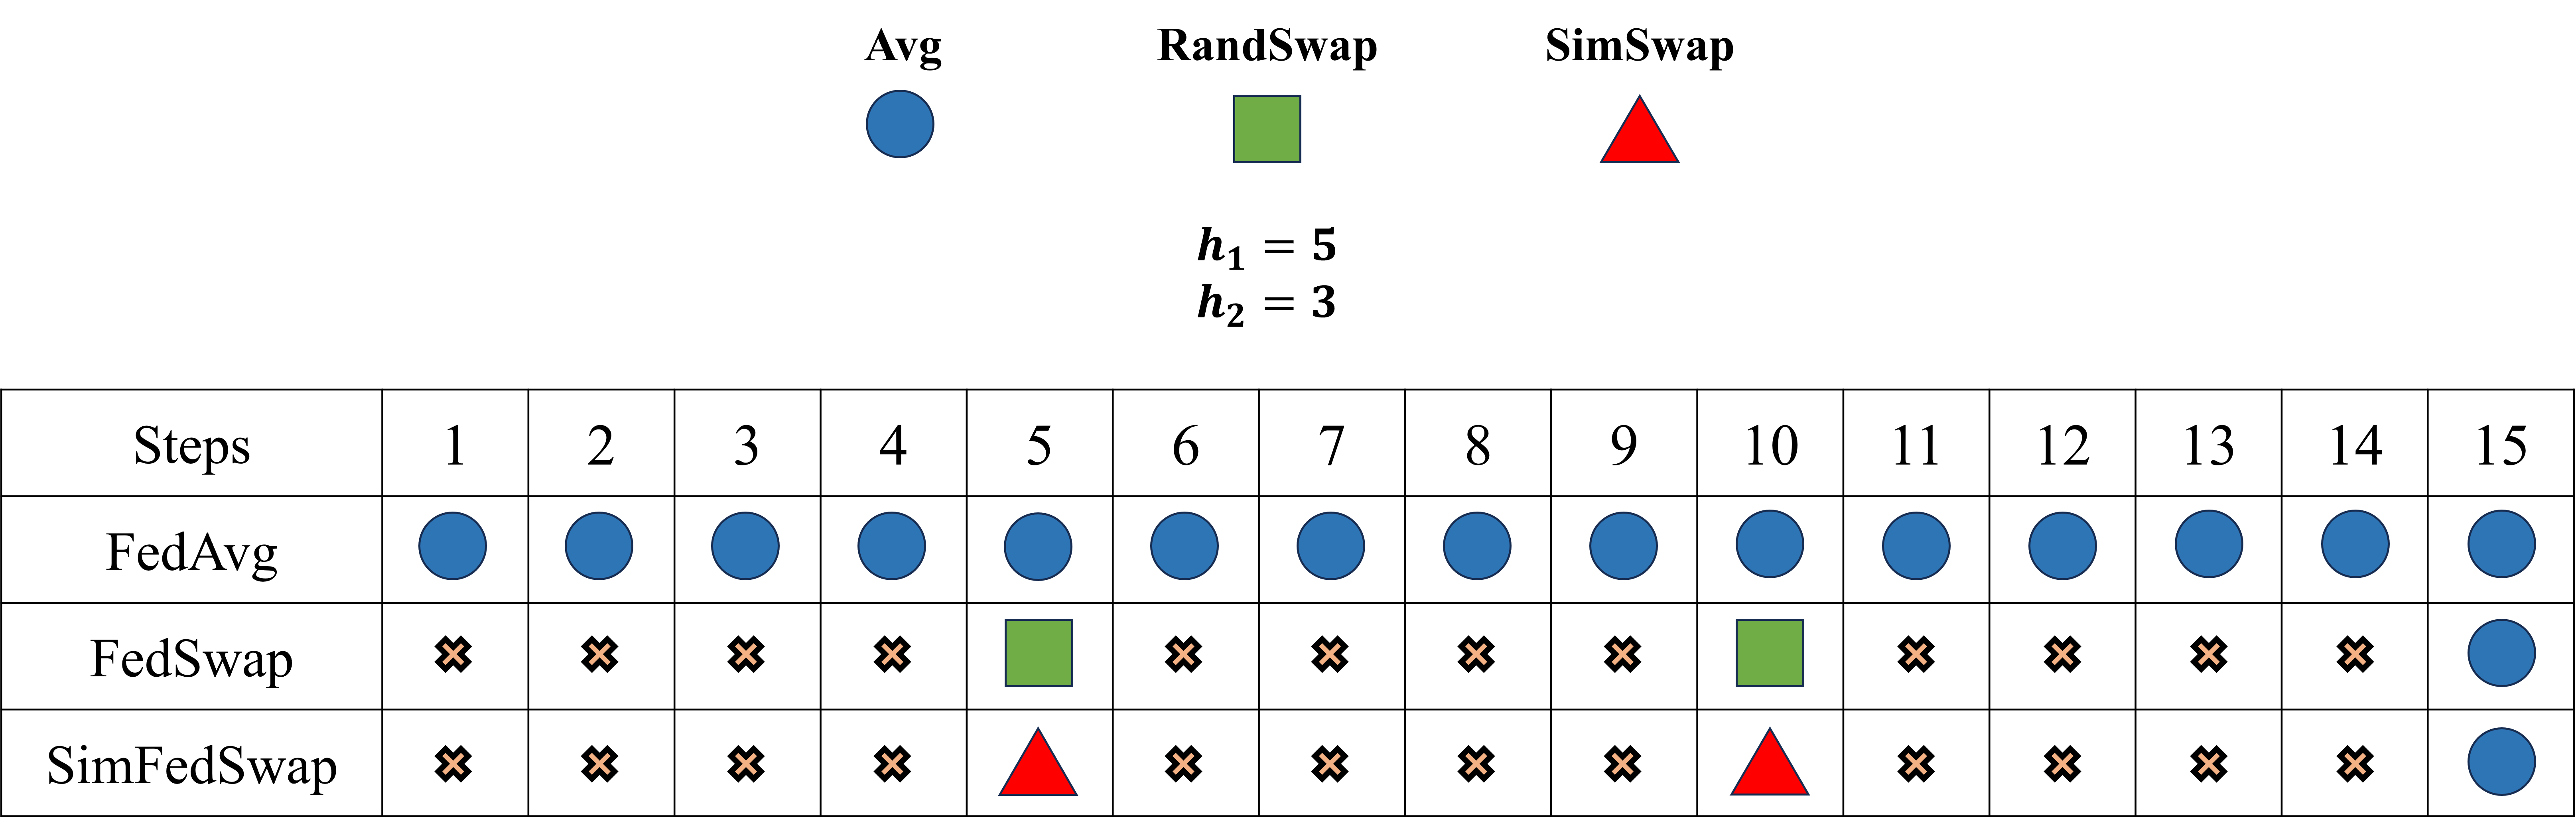
\includegraphics[scale=0.3]{images/chap4/compare_swap_net_traffic.png}%
	\caption{%
		تأثیر نحوه جابه‌جایی مدل‌ها بر ترافیک شبکه.
	}
	\label{compare_swap_net_traffic}
	\centering
\end{figure}
به‌طور خاص، در شبیه‌سازی‌هایی که پارامترهای \(h_1\) برابر با 5 و \(h_2\) برابر با 3 در نظر گرفته شده‌اند، روش \lr{FedSwap} موفق به کاهش
۸۶٫۶۶
درصدی هزینه‌های شبکه شده است. همچنین، روش \lr{SimFedSwap} توانسته این هزینه‌ها را تا ۸۰ درصد کاهش دهد. 


\subsection{
	تاثیر جابجایی مدل‌ها بر حریم شخصی در ارتباط بین سرور و کاربران
}
در روش یادگیری فدرال سنتی، مانند
\lr{FedAvg}%
، مدل‌ها پس از آموزش محلی توسط کاربران، به سرور مرکزی ارسال می‌شوند. سرور وظیفه تجمیع این مدل‌ها را بر عهده دارد و سپس مدل به‌روزرسانی‌ شده را به کاربران بازمی‌گرداند. در این روش، تعاملات فقط بین سرور و کاربران صورت می‌گیرد و هیچ ارتباط مستقیمی بین کاربران وجود ندارد. این امر باعث می‌شود که حریم شخصی کاربران به دلیل عدم تبادل مستقیم اطلاعات با یکدیگر، تا حد زیادی حفظ شود. همچنین کاربران نیازی به اعتماد به یکدیگر ندارند و تنها باید به سرور مرکزی اعتماد کنند.

در مقابل، در روش‌هایی که مدل‌ها بین خود کاربران جابه‌جا می‌شود، چه با واسطه سرور و چه بدون واسطه آن، خطرات بیشتری برای حریم شخصی وجود دارد. زمانی که مدل‌ها مستقیماً بین کاربران مبادله می‌شود، احتمال این که یکی از کاربران بتواند از طریق تحلیل مدل دریافت ‌شده اطلاعاتی در مورد داده‌های دیگر کاربران به دست آورد، افزایش می‌یابد. حتی اگر سرور به عنوان واسطه در این جابجایی‌ها عمل کند، همچنان خطراتی وجود خواهد داشت، زیرا سرور می‌تواند نقش ناظر را داشته باشد و از جابجایی مدل‌ها بین کاربران سوء استفاده کند. بنابراین، در هر دو حالت، جابجایی مدل‌ها بین کاربران نسبت به
\lr{FedAvg}
با چالش‌های بیشتری در زمینه حفظ حریم شخصی مواجه است.

در نتیجه، در روش
\lr{FedAvg}%
، به دلیل عدم ارتباط مستقیم بین کاربران، حریم شخصی به شکل بهتری حفظ می‌شود و تنها سرور مرکزی باید ایمن باشد. اما در روش جابجایی مدل‌ها بین کاربران، خطر نشت اطلاعات بین کاربران افزایش می‌یابد و این روش به پروتکل‌های امنیتی پیچیده‌تر و اعتماد بیشتر بین کاربران نیاز دارد.


\subsection{
	تاثیر جابجایی مدل‌ها بر حریم شخصی با توجه به واسطه بودن سرور
}
روش حریم خصوصی تفاضلی که در
\ref{privacy_challenge}
نیز به آن اشاره شد یکی از تکنیک‌های موثر برای حفظ حریم شخصی است که با اضافه کردن نویز به داده‌ها یا مدل‌ها، مانع از افشای اطلاعات حساس فردی می‌شود. این روش تضمین می‌کند که خروجی یک الگوریتم یادگیری به اندازه کافی تصادفی است، به‌طوری‌که حضور یا عدم حضور یک نمونه داده خاص در مجموعه داده‌ها، تاثیری بر خروجی نهایی نداشته باشد.

حال اگر از این روش در جابجایی مدل‌ها بین کاربران استفاده شود، تفاوت‌هایی بین دو رویکرد با واسطه سرور و بدون واسطه سرور وجود خواهد داشت. در حالتی که سرور واسطه باشد، اعمال حریم خصوصی تفاضلی می‌تواند به کنترل و مدیریت نویز اضافه شده کمک کند و سرور می‌تواند نقش فعالی در تضمین این که مدل‌ها به درستی ناشناس‌ شده‌اند، ایفا کند. این امر باعث می‌شود که خطر نشت اطلاعات به دلیل واسطه‌گری سرور کاهش یابد. اما همچنان باید به سرور اعتماد کرد که این فرآیند را به درستی انجام دهد.

در رویکرد بدون واسطه سرور، اعمال حریم خصوصی تفاضلی چالش‌برانگیزتر است، زیرا کاربران به‌طور مستقل باید نویز لازم را به مدل‌های خود اضافه کنند و در عین حال مطمئن شوند که سطح مناسبی از حفظ حریم شخصی برقرار است. در این حالت، هرگونه خطا یا ناهماهنگی در اعمال حریم خصوصی تفاضلی ممکن است منجر به افشای اطلاعات حساس شود. همچنین، نبود یک ناظر مرکزی مانند سرور، کار را برای هماهنگی و اجرای صحیح این روش پیچیده‌تر می‌کند.

در نتیجه، در صورت استفاده از روش حریم خصوصی تفاضلی، رویکرد با واسطه سرور به دلیل نظارت و کنترل متمرکز، از لحاظ حفظ حریم شخصی مزیت بیشتری دارد. در مقابل، در رویکرد بدون واسطه سرور، چالش‌های بیشتری برای کاربران وجود دارد که می‌تواند منجر به کاهش اثربخشی حریم خصوصی تفاضلی شود. در نهایت، اعتماد به سرور و هماهنگی دقیق بین کاربران نقش کلیدی در تعیین سطح امنیت و حریم شخصی خواهد داشت.




\section{
	نحوه تعیین کاربران نهایی جهت جابه‌جایی مدل‌ها در روش
	\lr{\texttt{\fontspec{Times New Roman} SimFedSwap}}
}
زمانی که همه مدل‌های شبکه عصبی در سرور مرکزی قرار دارند، وظیفه سرور این است که تصمیم بگیرد کدام کاربران مدل‌های خود را با یکدیگر جابه‌جا کنند. برای انجام این کار، ابتدا باید مدل‌ها با یکدیگر مقایسه شوند تا میزان شباهت بین آن‌ها مشخص شود. سپس، بر اساس این شباهت‌ها تعیین می‌شود که کدام کاربران مدل‌های شبکه عصبی خود را با یکدیگر مبادله کنند، یا به عبارت دیگر، سرور مشخص می‌کند کدام مدل به کدام کاربر ارسال شود.

نکته مهمی که باید مد نظر قرار داد این است که فرآیند بررسی شباهت بین مدل‌های شبکه عصبی ممکن است زمان‌بر باشد. بنابراین، برای تصمیم‌گیری سریع درباره جابه‌جایی مدل‌ها، باید از روش‌های مؤثری استفاده شود. در ادامه، دو روش برای تعیین کاربران نهایی جهت جابه‌جایی مدل‌ها معرفی می‌شود.


\subsection{
	روش جابه‌جایی حریصانه%
	\LTRfootnote{Greedy Swapping}
	\lr{\texttt{\fontspec{Times New Roman} (GS)}}
}\label{greedy_swapping}
در روش حریصانه، از بین تمام کاربران موجود، یک کاربر به‌صورت تصادفی انتخاب می‌شود. سپس مدل شبکه عصبی این کاربر با مدل‌های تمامی کاربران دیگر مقایسه می‌شود تا میزان شباهت آن‌ها سنجیده شود. در این مرحله، کاربری که مدل شبکه عصبی او کمترین شباهت را با مدل کاربر انتخاب‌ شده دارد، به عنوان کاربر مقصد برای جابه‌جایی مدل انتخاب می‌شود. پس از این انتخاب، سرور مدل‌های این دو کاربر را با یکدیگر جابه‌جا می‌کند و در نهایت این دو کاربر را از لیست انتخاب حذف خواهد کرد.

پس از انجام این جابه‌جایی، فرایند مشابهی برای کاربران باقی‌مانده تکرار می‌شود. ابتدا یک کاربر دیگر به‌صورت تصادفی انتخاب می‌شود و دقیقا همان روند بالا برای آن تکرار خواهد شد.
شبه کد کامل این روش در الگوریتم
\ref{algo_greedy_swapping}
ارائه شده است. علاوه بر این، نمادهای مختص به این الگوریتم در جدول
\ref{tabel_GreedySwappingNotations}
و همچنین تمامی نمادهای پایه در جدول
\ref{tabel_FedAvgNotations}
توضیح داده شده‌اند.
هدف از این جداول، فراهم کردن درکی جامع از نحوه عملکرد و پیاده‌سازی الگوریتم می‌باشد.


\begin{LTR}
	\SetAlgoNlRelativeSize{-1}
	\begin{algorithm}[t]
		\begin{RTL}
			\caption{%
				جابه‌جایی حریصانه
				\lr{(Greedy Swapping)}
			}
			\label{algo_greedy_swapping}
		\end{RTL}
		
		\begin{latin}
			\SetKwFunction{GreedySwapping}{GreedySwapping}
			\SetKwProg{Fn}{Function}{:}{end}
			\Fn{\GreedySwapping{}}{
				$LRS$ = copy of $U_t$\;
				$NS$ = (length of $U_t$ // 2) * $SP$\;
				\BlankLine
				
				\For{$NS$ times}{
					$RandomIndex$ = random integer between $0$ and length of $LRS$\;
					$SCB = LRS[RandomIndex]$\;
					remove $SCB$ from $LRS$\;
					
					\BlankLine
					Initialize $LstSimilarity$ as an empty list\;
					\For{each $RC \in LRS$}{
						$Sim = \texttt{ModelSimilarity} (w^{SCB}, w^{RC})$\;
						Append $Sim$ to $LstSimilarity$\;
					}
					$MinSimilarityIndex$ = index of the minimum value in $LstSimilarity$\;
					$SCD = LRS[MinSimilarityIndex]$\;
					remove $SCD$ from $LRS$\;
					\BlankLine
					
					$\texttt{Swap}(SCB, SCD)$\;
				}
			}
		\end{latin}
	\end{algorithm}
\end{LTR}


\begin{table}[h]
	\centering
	\caption{نمادهای مختص الگوریتم جابه‌جایی حریصانه}
	\label{tabel_GreedySwappingNotations}
	\begin{tabular}{cr}
		\hline
		متغیر & توضیحات \\
		\hline
		$LRS \, (LstRemainSwap)$ & لیست باقی‌مانده جابه‌جایی \\
		$NS \, (NumSwaps)$ & تعداد جابه‌جایی‌ها \\
		$SP \, (SwapPercentage)$ & ضریب کنترلی برای تعداد جابه‌جایی‌ها \\
		$RandomIndex$ & شاخص تصادفی \\
		$SCB \, (SwapClientBase)$ & کاربر مبدا جابه‌جایی \\
		$LstSimilarity$ & لیست مشابهت \\
		$RC \, (RemainClient)$ & کاربر باقی‌مانده \\
		$Sim$ & معیار مشابهت بین دو مدل شبکه عصبی \\
		$SCD \, (SwapClientDest)$ & کاربر مقصد جابه‌جایی
	\end{tabular}
\end{table}



در ادامه این مورد بررسی خواهد شد که تابع
\lr{ModelSimilarity}
در الگوریتم
\ref{algo_greedy_swapping}
چند مرتبه اجرا می‌شود. 
برای ساده‌تر کردن موضوع و فهم بهتر آن، لیست ‎\(LRS\) با \( n \) مقدار اولیه در نظر گرفته می‌شود (لیستی با \( n \) عضو) و همچنین مقدار \( NS \) برابر \( n/2 \) لحاظ خواهد شد. دلیل این انتخاب این است که با انجام \( n/2 \) جابه‌جایی، همه مدل‌ها یک بار جابه‌جا می‌شوند.
سپس حلقه اصلی به تعداد \( NS \) تکرار می‌شود. در هر تکرار از این حلقه یک عنصر تصادفی از \( LRS \) انتخاب و حذف خواهد شد. سپس برای هر عنصر باقی‌مانده در \( LRS \)، تابع
\lr{ModelSimilarity}
فراخوانی می‌شود.

تعداد تکرارهای حلقه داخلی که در آن تابع
\lr{ModelSimilarity}
فراخوانی می‌شود وابسته به تعداد عناصر باقی‌مانده در \( LRS \) است. به‌طور دقیق‌تر، در اولین تکرار حلقه اصلی، \( LRS \) شامل \(n-1\) عنصر است و در دومین تکرار، \( LRS \) شامل \(n-3\) عنصر خواهد بود; زیرا در هر تکرار از حلقه اصلی، یک عنصر به‌صورت تصادفی و یک عنصر دیگر با کمترین شباهت حذف می‌شوند.

به این ترتیب، تعداد کل فراخوانی‌های تابع
\lr{ModelSimilarity}
برابر است با مجموع تعداد عناصر باقی‌مانده در هر تکرار از حلقه اصلی:
\begin{equation}
	\sum_{i=0}^{NS-1} (n-1-2i)
\end{equation}
که این مجموع برای \( NS=n/2 \) به‌صورت زیر است:
\begin{equation}
	\sum_{i=0}^{(n/2)-1} (n-1-2i)
\end{equation}
این یک دنباله حسابی با مقدار اولیه \(a=n-1\) و قدر نسبت
 \(d=-2\) 
است و تعداد جملات آن برابر با \( NS \) است.
مجموع این دنباله حسابی به‌صورت زیر محاسبه می‌شود:
\begin{equation}
	S = NS \times \left( \frac{a+l}{2} \right)
\end{equation}
که در آن \( l \) مقدار آخرین جمله است و به این شکل به دست می‌آید:
\begin{equation}
	\begin{align*} 
		l &= n-1-2(NS-1) \\
		  &= n-1-2(n/2-1) \\
		  &= n-1-n+2 \\
		  &= 1
	\end{align*}
\end{equation}
بنابراین مجموع نهایی به این صورت خواهد بود:
\begin{equation}
	\begin{align*} 
		S &= (n/2) \times \left( \frac{(n-1)+1}{2} \right) \\
		&= (n/2) \times \left( \frac{n}{2} \right) \\
		&= \frac{n^2}{4}
	\end{align*}
\end{equation}
پس در نهایت تابع
\lr{ModelSimilarity}
به تعداد
\(
\floor{\frac{n^2}{4}}
 \) 
بار اجرا می‌شود.


\subsection{
مرتبه زمانی روش جابه‌جایی حریصانه
}\label{order_GS}
بر اساس فرضیات مطرح شده در بخش قبل، زمان اجرای الگوریتم جابه‌جایی حریصانه معادل \( O(kn^2) \) است.
باید توجه داشت که هنگام محاسبه مرتبه زمانی، مدت زمان اجرای تابع \lr{ModelSimilarity} برابر \( k \) در نظر گرفته شده است. این مقدار به معیار شباهتی که برای این تابع انتخاب می‌شود بستگی دارد و با توجه به نوع معیار، می‌تواند کاملا متفاوت باشد.


همچنین با توجه به این‌که مقدار \( NS \) برابر با \( n/2 \) فرض شده و هر بار اجرای حلقه اصلی شامل یک حذف از لیست \( LRS \) می‌شود که زمان اجرای آن \( O(n) \) است و با در نظر گرفتن این‌که حلقه داخلی نیز، طبق بررسی‌های انجام‌شده در بخش
\ref{greedy_swapping}،
مرتبه زمانی \( O(n) \) دارد، می‌توان نتیجه گرفت که ترکیب این دو عامل موجب می‌شود که کل زمان اجرای الگوریتم برابر با \( O(kn^2) \) باشد.
البته نکته مهم این است که محاسبات حلقه دوم می‌توانند به‌طور کامل به‌صورت موازی انجام شوند. به‌طور دقیق‌تر، عناصر موجود در لیست 
\lr{$LstSimilarity$} 
به یکدیگر وابستگی ندارند و می‌توان تمام آن‌ها را به‌طور همزمان محاسبه کرد. اگر سرور قابلیت اجرای موازی این عملیات را داشته باشد، محاسبه حلقه داخلی عملاً لحاظ نمی‌شود و مرتبه زمانی برابر
\( O(kn) \) 
خواهد شد. 


در نهایت، میزان مصرف حافظه توسط لیست
 \lr{$LstSimilarity$} 
در الگوریتم
 \ref{algo_greedy_swapping} 
بررسی می‌شود. همان‌طور که در بخش قبل توضیح داده شد، حلقه داخلی این الگوریتم در بیشترین حالت به تعداد \(n-1\) مرتبه اجرا می‌شود. بنابراین، از نظر حافظه، لیست
 \lr{$LstSimilarity$} 
در مرتبه \(O(n)\) قرار دارد. با این حال، باید توجه داشت که برای یافتن کمترین مقدار در یک مجموعه، حافظه‌ای به میزان \(O(1)\) نیز کافی است. 

در این الگوریتم، استفاده از لیست
 \lr{$LstSimilarity$} 
به منظور افزایش خوانایی و سادگی کد صورت گرفته است، اگرچه از لحاظ بهینه‌سازی حافظه می‌توان از روش‌های کم‌حافظه‌تری نیز استفاده کرد. به بیان دیگر، به‌جای نگهداری همه شباهت‌ها در یک لیست و سپس پیدا کردن کمترین مقدار، می‌توان به‌صورت مستقیم در همان حلقه داخلی کمترین شباهت را دنبال کرد و در هر تکرار، فقط مقدار کمینه فعلی را به‌روزرسانی کرد. این روش نیاز به حافظه کمتری دارد و با حافظه \(O(1)\) قابل انجام است.

با این حال، استفاده از لیست
 \lr{$LstSimilarity$} 
در این‌جا به منظور ساده‌تر و قابل فهم‌تر کردن کد انجام شده است. این انتخاب به توسعه‌دهندگان امکان می‌دهد تا الگوریتم را بهتر درک کنند و روند مقایسه شباهت‌ها را به وضوح مشاهده کنند، با این شرط که بهینه‌سازی حافظه در اولویت نباشد.




\subsection{
	روش جابه‌جایی حداقل شباهت%
	\LTRfootnote{Minimum Similarity Swapping}
	\lr{\texttt{\fontspec{Times New Roman} (MSS)}}
}
در این روش، برای این که حداقل شباهت ممکن بین تمامی مدل‌های شبکه عصبی به دست آید، لازم است تمامی مدل‌ها با یکدیگر مقایسه شوند و دو مدلی که کمترین شباهت را دارند با هم جابه‌جا شوند. به عنوان مثال، اگر \( n \) مدل وجود داشته باشد، باید یک ماتریس \( n \times n \) برای بررسی میزان شباهت‌ها ایجاد شود. در این ماتریس، شباهت مدل 1 با مدل 2 برابر با شباهت مدل 2 با مدل 1 در نظر گرفته می‌شود. همچنین به دلیل این که مقایسه یک مدل با خودش بی‌معنی است، ماتریس نهایی به شکل یک ماتریس بالا مثلثی%
\LTRfootnote{Upper Triangular Matrix}
(بدون قطر اصلی) تبدیل می‌شود. به این صورت که تنها حدود نیمی از ماتریس، شامل شباهت‌های مورد نیاز برای مقایسه است. در نتیجه ماتریس مورد نظر به شکل زیر در خواهد آمد.
\begin{equation}
	\begin{bmatrix}
		\infty & a^{12} & a^{13} & \cdots & a^{1n} \\
		\infty & \infty & a^{23} & \cdots & a^{2n} \\
		\infty & \infty & \infty & \cdots & a^{3n} \\
		\vdots & \vdots & \vdots & \ddots & \vdots \\
		\infty & \infty & \infty & \cdots & \infty
	\end{bmatrix}
	\label{eq_similarity_matrix}
\end{equation}

ابتدا، تمامی شباهت‌ها بین مدل‌ها محاسبه می‌شود و سپس از ماتریس ایجاد شده، کمترین مقدار شباهت انتخاب می‌شود. شماره سطر و ستون متناظر با این مقدار نشان می‌دهد که این دو مدل باید با یکدیگر جابه‌جا شوند. پس از انجام این جابه‌جایی، تمامی مقدارهای مربوط به سطر و ستون متناظر با این دو مدل باید به بی‌نهایت تغییر داده شوند تا در مراحل بعدی مجدد انتخاب نشوند. همچنین باید دقت کرد که هر دو سطر و ستون مرتبط با این دو مدل باید به بی‌نهایت تغییر داده شوند.

برای درک بهتر، فرض کنید کمترین مقدار شباهت در سطر سوم و ستون ششم ماتریس قرار دارد. در این حالت، مدل‌های سوم و ششم باید با یکدیگر جابه‌جا شوند. پس از این جابه‌جایی، لازم است که تمامی مقادیر در سطرهای سوم و ششم و همچنین ستون‌های سوم و ششم به بی‌نهایت تغییر کنند تا این دو مدل دیگر مورد بررسی قرار نگیرند. به این ترتیب، در دور بعدی، کوچک‌ترین مقدار شباهت از ماتریس انتخاب می‌شود و چون مقادیر مربوط به مدل‌های سوم و ششم به بی‌نهایت تغییر کرده‌اند، دیگر در این مرحله حضور نخواهند داشت و انتخاب نمی‌شوند. شبه کد کامل این روش در الگوریتم
\ref{algo_min_similarity_swapping}
ارائه شده است. علاوه بر این، نمادهای مختص به این الگوریتم در جدول
\ref{tabel_MinSimilaritySwapNotations}
توضیح داده شده‌اند.


\begin{LTR}
	\SetAlgoNlRelativeSize{-1}
	\begin{algorithm}[t]
		\begin{RTL}
			\caption{%
				جابه‌جایی حداقل شباهت
				\lr{(Minimum Similarity Swapping)}
			}
			\label{algo_min_similarity_swapping}
		\end{RTL}
		
		\begin{latin}
			\SetKwFunction{MinSimilaritySwapping}{MinSimilaritySwapping}
			\SetKwProg{Fn}{Function}{:}{end}
			\Fn{\MinSimilaritySwapping{}}{
				Initialize $SimArray$\;
				$L$ = length of $U_t$\;
				\BlankLine
				
				\For{each $row$ from $0$ to $L$}{
					\For{each $col$ from $(row+1)$ to $L$}{
						$Sim = \texttt{ModelSimilarity} (w^{row}, w^{col})$\;
						Append $Sim$ to $SimArray$\;
					}
				}
				\BlankLine
				
				$NS$ = ($L$ // 2) * $SP$\;
				\For{$NS$ times}{
					$MI$ = index of minimum value in $SimArray$\;
					$row, col$ = find $row$ and $col$ number, based on $MI$\;					
					Set all values of $SimArray[row, col]$ to $\infty$\;
					\BlankLine
					
					$\texttt{Swap}(w^{row}, w^{col})$\;
				}
			}
		\end{latin}
	\end{algorithm}
\end{LTR}



\begin{table}[h]
	\centering
	\caption{نمادهای مختص الگوریتم جابه‌جایی حداقل شباهت}
	\label{tabel_MinSimilaritySwapNotations}
	\begin{tabular}{cr}
		\hline
		متغیر & توضیحات \\
		\hline
		$SimArray$ & آرایه مشابهت \\
		$L$ & طول مجموعه‌ای از کاربران در گام $t$ \\
		$MI \, (MinIndex)$ & شاخص مقدار کمینه در آرایه مشابهت \\
		$row$ & شماره سطر بر اساس دید ماتریس مشابهت \\
		$col$ & شماره ستون بر اساس دید ماتریس مشابهت
	\end{tabular}
\end{table}




در این الگوریتم، تعداد دفعات اجرای تابع
\lr{ModelSimilarity}
به تعداد کل جابه‌جایی‌ها بین کاربران نهایی وابسته نیست. همان‌طور که در الگوریتم
\ref{algo_min_similarity_swapping}
مشاهده می‌شود، ماتریس شباهت تنها یک بار محاسبه خواهد شد. با توجه به ساختار ماتریس بالا مثلثی در رابطه
\ref{eq_similarity_matrix}
و با فرض این که تعداد مدل‌های کاربران برابر \(n\) در نظر گرفته شود، مقدار \(L\) در الگوریتم نیز برابر \(n\) خواهد شد.
در نتیجه، تعداد دفعات اجرای تابع
\lr{ModelSimilarity}
در الگوریتم جابه‌جایی حداقل شباهت، برابر با \(\frac{n(n-1)}{2}\) خواهد بود.


\subsection{
مرتبه زمانی و نحوه پیاده‌سازی روش جابه‌جایی حداقل شباهت
}
بر اساس فرضیات مطرح‌شده در بخش قبلی، زمان اجرای الگوریتم جابه‌جایی حداقل شباهت برابر با \( O(kn^2 + n^3) \) است. همچنین، مطابق با آنچه در بخش
\ref{order_GS}
بیان شد، مرتبه زمانی تابع
\lr{ModelSimilarity}
برابر
$k$
در نظر گرفته شده و طبق فرضیات بخش قبل، این تابع به تعداد \( O(n^2) \) بار اجرا می‌شود. بنابراین، بخش اول محاسبات با مرتبه زمانی \( O(kn^2) \) مشخص می‌شود.


برای محاسبات بخش دوم، پیدا کردن عنصر کمینه در ماتریس مشابهت، خود از مرتبه زمانی \(O(n^2)\) است. بنابراین، وقتی که حلقه اصلی \(n/2\) بار اجرا شود و هر بار نیاز به پیدا کردن عنصر کمینه در ماتریس مشابهت داشته باشد، مرتبه زمانی بخش دوم الگوریتم برابر \(O(n^2) \times O(n/2)\) خواهد بود که به \(O(n^3)\) ساده‌سازی می‌شود.
پس با ترکیب بخش اول و بخش دوم مرتبه زمانی کل الگوریتم برابر
\( O(kn^2 + n^3) \) 
خواهد شد.


لازم به ذکر است که محاسبات هر یک از عناصر ماتریس مشابهت، مستقل از یکدیگر هستند. اگر سرور قابلیت اجرای موازی این عملیات را داشته باشد، مرتبه زمانی محاسبه بخش اول برابر
\( O(k) \) 
و در نتیجه کل الگوریتم برابر با
\( O(k + n^3) \)
خواهد شد.


ماتریس مشابهت، در حالت عادی، دارای \(n^2\) عنصر است.
با بررسی دقیق‌تر الگوریتم و تعداد اجراهای حلقه دوم، در صورتی که از ماتریس مشابهت در پیاده‌سازی استفاده شود، از نظر زمان اجرا رابطه زیر به دست می‌آید:
\begin{equation}
	\begin{align*} 
		\left(\frac{n}{2}\right) \times (n^2 + 4n) &= \left(\frac{n^3}{2}\right)+2n^2 \\
		 &\xlongequal{\times 4} 2n^3 + 8n^2
	\end{align*}
\end{equation}
در این رابطه، تعداد اجراهای حلقه دوم برابر \(n/2\)، پیداکردن مقدار کمینه در ماتریس مشابهت برابر با \(n^2\) و انتساب مقدار بی‌نهایت برای دو سطر و ستون ماتریس مشابهت برابر با \(4n\) است.

با توجه به رابطه
\ref{eq_similarity_matrix}،
بیش از نصف ماتریس، شامل مقادیر بی‌نهایت می‌باشد. بنابراین، با پیاده‌سازی ماتریس به‌صورت یک آرایه یک‌بعدی و تنها ذخیره‌سازی مقادیر بالا مثلثی، می‌توان با انجام چند عملیات ساده ریاضی به مقدار سطر و ستون مورد نظر در ماتریس مشابهت دست یافت.

در این پیاده‌سازی، آرایه یک‌بعدی جدید دارای \(\frac{n(n-1)}{2}\) عنصر خواهد بود. اگر حلقه دوم الگوریتم، مجدد بررسی شود، زمان اجرای آن به‌صورت زیر خواهد بود:
\begin{equation}
	\begin{align*} 
		\left(\frac{n}{2}\right) \times \left(\frac{n(n-1)}{2} + 4n\right) &= \left(\frac{n^2(n-1)}{4} \right)+2n^2 \\
		&= \left(\frac{n^3}{4} - \frac{n^2}{4}\right) +2n^2 \\
		&\xlongequal{\times 4} n^3-n^2+8n^2 \\
		&= n^3+7n^2
	\end{align*}
\end{equation}
در این عبارت، تعداد اجراهای حلقه دوم برابر \(n/2\)، پیداکردن مقدار کمینه در آرایه برابر \(\frac{n(n-1)}{2}\) و در نهایت انتساب مقدار بی‌نهایت در آرایه مربوطه برابر با \(4n\) خواهد بود.

همان‌طور که مشاهده می‌شود، این پیاده‌سازی تقریبا سرعت اجرای الگوریتم را دو برابر می‌کند. اگرچه از نظر مرتبه زمانی بهبودی حاصل نشد، اما افزایش سرعت اجرا به میزان دو برابر، بهبود قابل توجهی در روند آموزش محسوب می‌شود. همچنین از نظر حافظه نیز بهبود حاصل شده است، زیرا در صورت استفاده از ماتریس مشابهت نیاز به ذخیره‌سازی \(n^2\) عنصر است، در حالی که با به‌کارگیری آرایه مشابهت تنها \(\frac{n(n-1)}{2}\) عنصر ذخیره خواهد شد. بنابراین، استفاده از ساختار آرایه یک بعدی می‌تواند بسیار مفید بوده و به کارایی الگوریتم کمک کند.




\section{جمع‌بندی}

روش جابه‌جایی فدرال به‌جای ادغام مدل‌های محلی در هر مرحله از یادگیری فدرال، این مدل‌ها را بین دستگاه‌ها جابه‌جا می‌کند. این روش با هدف کاهش تأثیرات منفی ناشی از داده‌های
\lr{non-IID}
و بهبود دقت مدل‌ها طراحی شده است. جابه‌جایی مدل‌ها به دستگاه‌های مختلف اجازه می‌دهد تا به داده‌های متنوع‌تری دسترسی پیدا کنند و عملکرد مدل سراسری بهبود یابد. همچنین، جابه‌جایی فدرال در دو حالت تصادفی و بر پایه شباهت معرفی شد که در حالت دوم، مدل‌هایی که کمترین شباهت را دارند جابه‌جا می‌شوند تا تنوع داده‌ها افزایش یابد و یادگیری بهینه‌تر صورت گیرد.


جابه‌جایی مدل‌ها در روش‌های
\lr{FedSwap}
و
\lr{SimFedSwap}
می‌تواند هزینه‌های ارتباطی را به میزان قابل‌توجهی کاهش دهد و از این نظر بر ترافیک شبکه تاثیر مثبتی داشته باشد. از سوی دیگر، این جابه‌جایی‌ها می‌توانند چالش‌های جدیدی را در زمینه حفظ حریم شخصی ایجاد کنند، به ویژه زمانی که مدل‌ها مستقیما بین کاربران جابه‌جا می‌شوند. استفاده از روش‌های حریم خصوصی تفاضلی می‌تواند به کاهش این خطرات کمک کند، اما اجرای صحیح آن‌ها، به ویژه بدون واسطه‌گری سرور، چالش ‌برانگیز است.


برای حفظ دقت در مقایسه‌های شبکه‌های عصبی در شرایط مختلف، لازم است شاخص‌های شباهت در برابر تغییرات مقاوم باشند. برای تحلیل عمیق‌تر، استفاده از روش‌های مختلفی مانند معیارهای نرمال‌شده یا همان
\lr{CKA}
پیشنهاد می‌شود. ارزیابی لایه‌های شبکه به‌صورت جداگانه و ترکیب نتایج آن‌ها به بهینه‌سازی شاخص انتخاب شده کمک می‌کند. در نهایت، در روش
\lr{SimFedSwap}%
، سرور دو مدل با کمترین شباهت را انتخاب و با یکدیگر جابه‌جا می‌کند که این فرآیند بر اساس روش حریصانه یا حداقل شباهت انجام می‌گیرد.

